\documentclass{beamer}
% =============================================================================
% ENCODING
% =============================================================================
\usepackage[utf8]{inputenc}  % UTF-8 encoding support

% =============================================================================
% GRAPHICS
% =============================================================================
\usepackage{graphicx}  % For \includegraphics (401 uses across lectures)

% =============================================================================
% MATH PACKAGES
% =============================================================================
\usepackage{amsmath}    % For align, multline, equation environments (heavily used)
\usepackage{amsfonts}   % For \mathbb (e.g., \bbR, \bbE)
\usepackage{amssymb}    % For additional math symbols

% =============================================================================
% TABLES
% =============================================================================
\usepackage{booktabs}   % For \toprule, \midrule, \bottomrule (used in lecture13, lecture14)

% =============================================================================
% LISTS
% =============================================================================
\usepackage{enumerate}  % Enhanced enumerate environment (76 uses across lectures)

% =============================================================================
% TIKZ (DIAGRAMS)
% =============================================================================
\usepackage{tikz}       % For taxonomy diagram and footnotes positioning

% =============================================================================
% UTILITY PACKAGES
% =============================================================================
\usepackage{multido}    % For \multido command used in \eqpause
\usepackage{etoolbox}   % For \AtEndEnvironment, \ifbool, \newbool (used in preamble and taxonomy)
\usepackage{xspace}     % For smart spacing after custom commands (\ODESolve, \SDESolve)

% =============================================================================
% BEAMER THEME SETTINGS
% =============================================================================
\usetheme{default}
\usecolortheme{default}

\setbeamerfont{title}{size=\Huge}
\setbeamertemplate{footline}[frame number]{}
\setbeamertemplate{section in toc}[sections numbered]

\makeatletter
\newcommand\HUGE{\@setfontsize\Huge{35}{40}}
\makeatother    

\setbeamerfont{title}{size=\HUGE}
\beamertemplatenavigationsymbolsempty

% =============================================================================
% TIKZ LIBRARIES
% =============================================================================
% Used for taxonomy diagram: arrows, positioning, shapes
\usetikzlibrary{arrows.meta,calc,shapes,positioning,shadows,trees}

% =============================================================================
% CUSTOM FOOTNOTE COMMANDS
% =============================================================================
% \myfootnote{text} - creates a footnote at the bottom of the slide
\newcommand\myfootnote[1]{%
  \vspace{-0.5cm}%
  \tikz[remember picture,overlay]
  \draw (current page.south west) +(1in + \oddsidemargin,0.5em)
  node[anchor=south west,inner sep=0pt]{\parbox{\textwidth}{%
      \rlap{\rule{10em}{0.4pt}}\raggedright\scriptsize \textit{#1}}};}

% \myfootnotewithlink{url}{text} - creates a clickable footnote (623 uses across lectures)
\newcommand\myfootnotewithlink[2]{%
  \vspace{-0.5cm}%
  \tikz[remember picture,overlay]
  \draw (current page.south west) +(1in + \oddsidemargin,0.5em)
  node[anchor=south west,inner sep=0pt]{\parbox{\textwidth}{%
      \rlap{\rule{10em}{0.4pt}}\raggedright\scriptsize\href{#1}{\textit{#2}}}};}

% =============================================================================
% SECTION/SUBSECTION OUTLINE AUTOMATION
% =============================================================================
% Automatically show outline at the beginning of each section
\AtBeginSection[]
      {
      	\begin{frame}{Outline}
      		\tableofcontents[currentsection]
      	\end{frame}
      }
      \AtBeginSubsection[]{
      	\begin{frame}{Outline}
      		\tableofcontents[currentsection,currentsubsection]
      	\end{frame}
}

% =============================================================================
% CUSTOM SLIDE ANIMATION COMMANDS
% =============================================================================
% These commands enable step-by-step reveal of equations and content
% Used heavily across all lectures (1130+ uses of \nextonslide and \eqpause)

\newcounter{noscounter}   % Counter for \nextonslide (resets on each new slide)
\newcounter{pcounter}     % Counter for pause commands (resets after \eqpause)
\newcounter{diffcounter}  % Counts pauses after equations

% \nextonslide{content} - reveals content on the next overlay
\newcommand{\nextonslide}[1]{%
  \stepcounter{noscounter}%
  \stepcounter{pcounter}%
  \stepcounter{diffcounter}%
  \onslide<\value{noscounter}->{#1}%
}

% \resetonslide - resets all animation counters (called at each frame)
\newcommand{\resetonslide}{%
    \setcounter{noscounter}{1}%
    \setcounter{pcounter}{1}%
    \setcounter{diffcounter}{0}%
}

% \eqpause - pause after equation that syncs with \nextonslide
\newcommand{\eqpause}{%
  \multido{\i=1+1}{\value{pcounter}}{\pause}%
  \stepcounter{noscounter}%
  \setcounter{pcounter}{1}%
}

% \eqpausediff - helper command, runs automatically after math environments
\newcommand{\eqpausediff}{%
  \multido{\i=1+1}{\value{diffcounter}}{\pause}%
  \addtocounter{pcounter}{-\value{diffcounter}}%
  \setcounter{diffcounter}{0}%
}

% Apply \eqpausediff after math environments
\newcommand\AtEndBoth[2]{%
  \AtEndEnvironment{#1}{#2}%
  \AtEndEnvironment{#1*}{#2}%
}

\AtEndBoth{align}{\eqpausediff}
\AtEndBoth{equation}{\eqpausediff}
\AtEndBoth{multline}{\eqpausediff}

% Reset counters at the beginning of each frame
\addtobeamertemplate{frametitle}{\resetonslide}{}

% =============================================================================
% INCLUDE OTHER CONFIGURATION FILES
% =============================================================================
% ==============================================================================
% Custom LaTeX Commands for Deep Generative Models Course
% ==============================================================================

% ==============================================================================
% BOLD LETTERS (mathbf / boldsymbol)
% ==============================================================================

% ------------------------------------------------------------------------------
% Latin Bold Lowercase
% Usage: \bx for x in bold, commonly used for vectors
% ------------------------------------------------------------------------------
\newcommand{\ba}{\mathbf{a}}
\newcommand{\bc}{\mathbf{c}}
\newcommand{\be}{\mathbf{e}}
\newcommand{\bff}{\mathbf{f}}  % Note: \bf is reserved for bold font switching
\newcommand{\bg}{\mathbf{g}}
\newcommand{\bh}{\mathbf{h}}
\newcommand{\bp}{\mathbf{p}}
\newcommand{\bq}{\mathbf{q}}
\newcommand{\bs}{\mathbf{s}}
\newcommand{\bt}{\mathbf{t}}
\newcommand{\bu}{\mathbf{u}}
\newcommand{\bv}{\mathbf{v}}
\newcommand{\bw}{\mathbf{w}}
\newcommand{\bx}{\mathbf{x}}
\newcommand{\by}{\mathbf{y}}
\newcommand{\bz}{\mathbf{z}}
\newcommand{\bzero}{\boldsymbol{0}}  % Zero vector
\newcommand{\bone}{\mathbf{1}}       % Ones vector

% ------------------------------------------------------------------------------
% Latin Bold Uppercase
% Usage: \bX for X in bold, commonly used for matrices or random vectors
% ------------------------------------------------------------------------------
\newcommand{\bA}{\mathbf{A}}
\newcommand{\bG}{\mathbf{G}}
\newcommand{\bI}{\mathbf{I}}
\newcommand{\bJ}{\mathbf{J}}
\newcommand{\bL}{\mathbf{L}}
\newcommand{\bM}{\mathbf{M}}
\newcommand{\bP}{\mathbf{P}}
\newcommand{\bQ}{\mathbf{Q}}
\newcommand{\bR}{\mathbf{R}}
\newcommand{\bT}{\mathbf{T}}
\newcommand{\bU}{\mathbf{U}}
\newcommand{\bV}{\mathbf{V}}
\newcommand{\bW}{\mathbf{W}}
\newcommand{\bX}{\mathbf{X}}
\newcommand{\bZ}{\mathbf{Z}}

% ------------------------------------------------------------------------------
% Greek Bold Lowercase
% Usage: \btheta for θ in bold, commonly used for parameter vectors
% ------------------------------------------------------------------------------
\newcommand{\bepsilon}{\boldsymbol{\epsilon}}
\newcommand{\blambda}{\boldsymbol{\lambda}}
\newcommand{\bmu}{\boldsymbol{\mu}}
\newcommand{\bphi}{\boldsymbol{\phi}}
\newcommand{\bpi}{\boldsymbol{\pi}}
\newcommand{\bpsi}{\boldsymbol{\psi}}
\newcommand{\bsigma}{\boldsymbol{\sigma}}
\newcommand{\btheta}{\boldsymbol{\theta}}

% ------------------------------------------------------------------------------
% Greek Bold Uppercase
% Usage: \bSigma for Σ in bold, commonly used for covariance matrices
% ------------------------------------------------------------------------------
\newcommand{\bPhi}{\boldsymbol{\Phi}}
\newcommand{\bSigma}{\boldsymbol{\Sigma}}
\newcommand{\bTheta}{\boldsymbol{\Theta}}

% ==============================================================================
% CALLIGRAPHIC LETTERS (mathcal)
% Usage: \cX for calligraphic X, commonly used for sets and spaces
% ==============================================================================
\newcommand{\cF}{\mathcal{F}}
\newcommand{\cI}{\mathcal{I}}
\newcommand{\cL}{\mathcal{L}}
\newcommand{\cM}{\mathcal{M}}
\newcommand{\cN}{\mathcal{N}}
\newcommand{\cO}{\mathcal{O}}
\newcommand{\cP}{\mathcal{P}}
\newcommand{\cS}{\mathcal{S}}
\newcommand{\cT}{\mathcal{T}}
\newcommand{\cW}{\mathcal{W}}
\newcommand{\cX}{\mathcal{X}}
\newcommand{\cZ}{\mathcal{Z}}

% ==============================================================================
% BLACKBOARD BOLD LETTERS (mathbb)
% Usage: \bbR for ℝ, commonly used for number sets and expectations
% ==============================================================================
\newcommand{\bbE}{\mathbb{E}}  % Expectation
\newcommand{\bbI}{\mathbb{I}}  % Indicator function
\newcommand{\bbP}{\mathbb{P}}  % Probability measure
\newcommand{\bbR}{\mathbb{R}}  % Real numbers

% ==============================================================================
% MATH OPERATORS
% ==============================================================================

% ------------------------------------------------------------------------------
% Optimization Operators
% Usage: \argmin_{x} f(x) for proper spacing and limits placement
% ------------------------------------------------------------------------------
\DeclareMathOperator*{\argmin}{arg\,min}
\DeclareMathOperator*{\argmax}{arg\,max}

% ------------------------------------------------------------------------------
% Statistical Operators
% Usage: \cov(X, Y) for covariance
% ------------------------------------------------------------------------------
\DeclareMathOperator{\cov}{cov}

% ------------------------------------------------------------------------------
% Linear Algebra Operators
% Usage: \tr(\bA) for trace of matrix A
% ------------------------------------------------------------------------------
\DeclareMathOperator{\tr}{tr}

% ------------------------------------------------------------------------------
% Other Mathematical Operators
% ------------------------------------------------------------------------------
\DeclareMathOperator{\diver}{div}      % Divergence (vector calculus)
\newcommand{\sg}{\mathrm{sg}}          % Stop-gradient operator
\DeclareMathOperator{\softmax}{softmax}
\DeclareMathOperator{\supp}{supp}      % Support of a distribution

% ==============================================================================
% PROBABILITY DISTRIBUTIONS
% Usage: X \sim \cN(0, 1), Y \sim \Bern(p)
% ==============================================================================
\DeclareMathOperator{\Bern}{Bern}      % Bernoulli distribution
\DeclareMathOperator{\Cat}{Cat}        % Categorical distribution
\DeclareMathOperator{\Gumbel}{Gumbel}  % Gumbel distribution
\DeclareMathOperator{\Uniform}{Uniform}

% ==============================================================================
% METRICS AND DIVERGENCES
% Usage: \KL(p \| q), \JSD(p, q)
% ==============================================================================
\newcommand{\Ent}{\mathrm{H}}          % Entropy
\newcommand{\FID}{\mathrm{FID}}        % Fréchet Inception Distance
\newcommand{\JSD}{D_\mathrm{JS}}        % Jensen-Shannon Divergence
\newcommand{\KL}{D_\mathrm{KL}}        % Kullback-Leibler Divergence
\DeclareMathOperator{\MMD}{MMD}        % Maximum Mean Discrepancy
\DeclareMathOperator{\SNR}{SNR}        % Signal-to-Noise Ratio

% ==============================================================================
% NEURAL NETWORK NOTATION
% ==============================================================================

% ------------------------------------------------------------------------------
% Network Architectures (upright font for abbreviations)
% Usage: f_{\btheta} = \NN_{\btheta}(\bx)
% ------------------------------------------------------------------------------
\newcommand{\MLP}{\mathrm{MLP}}        % Multi-Layer Perceptron
\newcommand{\NN}{\mathrm{NN}}          % Neural Network
\newcommand{\RNN}{\mathrm{RNN}}        % Recurrent Neural Network

% ------------------------------------------------------------------------------
% Numerical Solvers (monospace font)
% Usage: \bx_T = \ODESolve(v, \bx_0, T)
% ------------------------------------------------------------------------------
\newcommand{\ODESolve}{\texttt{ODESolve}\xspace}
\newcommand{\SDESolve}{\texttt{SDESolve}\xspace}

% ==============================================================================
% COMMON SHORTCUTS
% Usage: Frequently used subscripted or parameterized expressions
% ==============================================================================
\newcommand{\pd}{p_{\text{data}}}              % Data distribution
\newcommand{\pt}{p_{\boldsymbol{\theta}}}      % Parameterized distribution
\newcommand{\qagg}{q_{\text{agg}}}             % Aggregated posterior
\newcommand{\lambdamax}{\lambda_{\text{max}}}  % Maximum eigenvalue
  % Math shorthand commands (\bx, \bbE, \KL, etc.)
\input{../utils/title}        % Title page template
% For each possible node, we create a boolean
\newbool{hl@root}
\newbool{hl@explicit}
\newbool{hl@implicit}
\newbool{hl@exact}
\newbool{hl@approx}
\newbool{hl@gan}
\newbool{hl@ar}
\newbool{hl@nf}
\newbool{hl@vae}
\newbool{hl@score}
\newbool{hl@cont}
\newbool{hl@ddpm}
\newbool{hl@sm}
\newbool{hl@ode}
\newbool{hl@sde}
\newbool{hl@fm}

% Command to reset all bools
\newcommand{\resetAllHighlights}{%
    \boolfalse{hl@root}%
    \boolfalse{hl@explicit}%
    \boolfalse{hl@implicit}%
    \boolfalse{hl@exact}%
    \boolfalse{hl@approx}%
    \boolfalse{hl@gan}%
    \boolfalse{hl@ar}%
    \boolfalse{hl@nf}%
    \boolfalse{hl@vae}%
    \boolfalse{hl@score}%
    \boolfalse{hl@cont}%
    \boolfalse{hl@ddpm}%
    \boolfalse{hl@sm}%
    \boolfalse{hl@ode}%
    \boolfalse{hl@sde}%
    \boolfalse{hl@fm}%
}

% Command to set a single highlight
\newcommand{\setHighlight}[1]{%
    \booltrue{hl@#1}%
}

% Command to set highlights from comma-separated list
\newcommand{\setHighlights}[1]{%
    \resetAllHighlights%
    \forcsvlist{\setHighlight}{#1}%
}

% Highlighted style definition
\tikzset{
    hl/.style={line width=1.2pt, draw=black, font=\scriptsize\bfseries},
    box/.style={
        rectangle, 
        draw=gray!50, 
        rounded corners=2pt, 
        minimum width=1.9cm, 
        minimum height=0.5cm, 
        align=center, 
        font=\scriptsize, 
        line width=0.4pt
    },
    rootnode/.style={box, fill=violet!20},
    category/.style={box, fill=teal!20},
    model/.style={box, fill=yellow!30},
    arrow/.style={-Stealth, draw=gray!80, line width=0.4pt}
}

% Draw taxonomy with pre-set highlights
\newcommand{\drawTaxonomy}{%
    \begin{tikzpicture}[scale=0.9, transform shape, node distance=0.6cm and 0.3cm]
        % --- CENTRAL ROOT ---
        \ifbool{hl@root}{\node[rootnode, hl] (root) {Generative Models};}{\node[rootnode] (root) {Generative Models};}

        % --- UPPER BRANCHES ---
        \ifbool{hl@explicit}{\node[category, hl, above left=0.6cm and 0.5cm of root] (explicit) {Explicit density};}{\node[category, above left=0.6cm and 0.5cm of root] (explicit) {Explicit density};}
        \ifbool{hl@implicit}{\node[category, hl, above right=0.6cm and 0.5cm of root] (implicit) {Implicit density};}{\node[category, above right=0.6cm and 0.5cm of root] (implicit) {Implicit density};}

        \ifbool{hl@exact}{\node[category, hl, above left=0.6cm and -0.6cm of explicit] (exact) {Exact likelihood};}{\node[category, above left=0.6cm and -0.6cm of explicit] (exact) {Exact likelihood};}
        \ifbool{hl@approx}{\node[category, hl, above right=0.6cm and -0.6cm of explicit] (approx) {Approximate likelihood};}{\node[category, above right=0.6cm and -0.6cm of explicit] (approx) {Approximate likelihood};}

        \ifbool{hl@gan}{\node[model, hl, above=0.6cm of implicit] (gans) {GANs};}{\node[model, above=0.6cm of implicit] (gans) {GANs};}

        \ifbool{hl@ar}{\node[model, hl, above left=0.6cm and -0.9cm of exact] (ar) {Autoregressive \\ models};}{\node[model, above left=0.6cm and -0.9cm of exact] (ar) {Autoregressive \\ models};}
        \ifbool{hl@nf}{\node[model, hl, above right=0.6cm and -0.9cm of exact] (nf) {Normalizing \\ Flows};}{\node[model, above right=0.6cm and -0.9cm of exact] (nf) {Normalizing \\ Flows};}
        \ifbool{hl@vae}{\node[model, hl, above=0.6cm of approx] (vae) {Variational \\ Autoencoders};}{\node[model, above=0.6cm of approx] (vae) {Variational \\ Autoencoders};}

        % --- LOWER BRANCHES ---
        \ifbool{hl@score}{\node[category, hl, below left=0.6cm and 0.5cm of root] (score) {Score-based};}{\node[category, below left=0.6cm and 0.5cm of root] (score) {Score-based};}
        \ifbool{hl@cont}{\node[category, hl, below right=0.6cm and 0.5cm of root] (cont) {Continuous \\ dynamics};}{\node[category, below right=0.6cm and 0.5cm of root] (cont) {Continuous \\ dynamics};}

        \ifbool{hl@sm}{\node[model, hl, below left=0.6cm and -0.8cm of score] (sm) {Score Matching};}{\node[model, below left=0.6cm and -0.8cm of score] (sm) {Score Matching};}
        \ifbool{hl@ddpm}{\node[model, hl, below right=0.6cm and -0.8cm of score] (ddpm) {Denoising Diffusion};}{\node[model, below right=0.6cm and -0.8cm of score] (ddpm) {Denoising Diffusion};}

        \ifbool{hl@ode}{\node[model, hl, below left=0.6cm and -0.8cm of cont] (ode) {Neural ODEs};}{\node[model, below left=0.6cm and -0.8cm of cont] (ode) {Neural ODEs};}
        \ifbool{hl@sde}{\node[model, hl, below right=0.6cm and -0.8cm of cont] (sde) {SDE-based \\ Diffusion};}{\node[model, below right=0.6cm and -0.8cm of cont] (sde) {SDE-based \\ Diffusion};}

        \ifbool{hl@fm}{\node[model, hl, below=0.6cm of ode] (fm) {Flow Matching};}{\node[model, below=0.6cm of ode] (fm) {Flow Matching};}

        % --- CONNECTIONS ---
        \draw[arrow] (root.north) -- ++(0,0.3) -| (explicit.south);
        \draw[arrow] (root.north) -- ++(0,0.3) -| (implicit.south);
        \draw[arrow] (root.south) -- ++(0,-0.3) -| (score.north);
        \draw[arrow] (root.south) -- ++(0,-0.3) -| (cont.north);
        \draw[arrow] (explicit.north) -- ++(0,0.3) -| (exact.south);
        \draw[arrow] (explicit.north) -- ++(0,0.3) -| (approx.south);
        \draw[arrow] (exact.north) -- ++(0,0.3) -| (ar.south);
        \draw[arrow] (exact.north) -- ++(0,0.3) -| (nf.south);
        \draw[arrow] (approx.north) -- (vae.south);
        \draw[arrow] (implicit.north) -- (gans.south);
        \draw[arrow] (score.south) -- ++(0,-0.3) -| (sm.north);
        \draw[arrow] (score.south) -- ++(0,-0.3) -| (ddpm.north);
        \draw[arrow] (cont.south) -- ++(0,-0.3) -| (ode.north);
        \draw[arrow] (cont.south) -- ++(0,-0.3) -| (sde.north);
        \draw[arrow] (ode.south) -- (fm.north);
    \end{tikzpicture}
}

% The main taxonomy rendering command
\newcommand{\renderTaxonomy}[1]{%
    \setHighlights{#1}%
    \centering
    \drawTaxonomy%
}     % Generative models taxonomy diagram

\createdgmtitle{10}

%--------------------------------------------------------------------------------
\begin{document}
%--------------------------------------------------------------------------------
\begin{frame}[noframenumbering,plain]
\titlepage
	\resetonslide	
\end{frame}
%=======
\begin{frame}{Recap of Previous Lecture}
	\myfootnotewithlink{https://arxiv.org/abs/1806.07366}{Chen R. T. Q. et al. Neural Ordinary Differential Equations, 2018}   
	\begin{block}{Continuous-Time Dynamics}
		\vspace{-0.5cm}
		\begin{align*}
			\frac{d \bx(t)}{dt} &= \bv_{\btheta}(\bx(t), t); \quad \text{with initial condition }\bx(t_0) = \bx_0. \\
			\bpsi_t(\bx_0) &= \int^{t}_{t_0} \bv_{\btheta}(\bx(s), s) d s  + \bx_0 \approx {\color{teal}\ODESolve_v(\bx_0, \btheta, t_0, t)}.
		\end{align*}
		\vspace{-0.5cm}
	\end{block}
	\begin{itemize}
		\item $\bv_{\btheta}: \bbR^m \times [t_0, t_1] \rightarrow \bbR^m$ is a vector field.
		\item $\bpsi: \bbR^m \times [t_0, t_1] \rightarrow \bbR^m$ is a flow (the solution of ODE):
	\end{itemize}
	\begin{block}{Euler \ODESolve}
		\vspace{-0.3cm}
		\[
  			\bx(t + h) = \bx(t) + h \cdot \bv_{\btheta}(\bx(t), t)
		\]
	\end{block}
	More advanced numerical methods (such as Runge-Kutta) are often used instead of unstable Euler update step.
\end{frame}
%=======
\begin{frame}{Recap of Previous Lecture}
	\myfootnotewithlink{https://arxiv.org/abs/1810.01367}{Grathwohl W. et al. FFJORD: Free-form Continuous Dynamics for Scalable Reversible Generative Models, 2018}  
	\vspace{-0.3cm}
	\[
 		\frac{d \bx(t)}{dt} = \bv_{\btheta}(\bx(t), t);\quad \bx(t_0) = \bx_0
	\]
	\vspace{-0.3cm}
	\begin{itemize}
		\item Suppose $\bx(0)$ is a random variable with density~$p_0(\bx)$. Then, $\bx(t)$ is a random variable with density~$p_t(\bx)$.
		\item $p_t(\bx) = p(\bx, t)$ describes the \textbf{probability path} between $p_0(\bx)$ and $p_1(\bx)$.
	\end{itemize}
	\vspace{-0.3cm}
	\begin{figure}
		\centering
		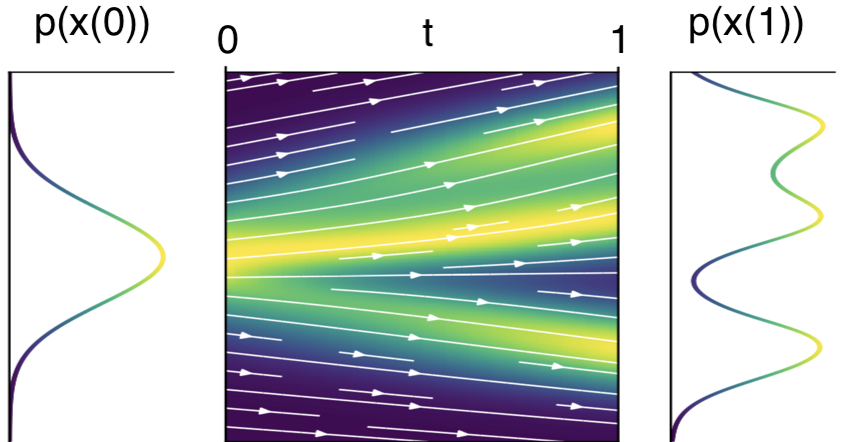
\includegraphics[width=0.7\linewidth]{figs/cnf_flow.png}
	\end{figure}
\end{frame}
%=======
\begin{frame}{Recap of Previous Lecture}
	\myfootnotewithlink{https://arxiv.org/abs/1806.07366}{Chen R. T. Q. et al. Neural Ordinary Differential Equations, 2018}   
	\begin{block}{Theorem (Picard)}
		If $\bv$ is continuously differentiable with a bounded derivative in $\bx$ and continuous in $t$, then the ODE has a \textbf{unique solution} given by a flow $\bpsi_t$.
	\end{block}
	This guarantees the ODE is \textbf{uniquely reversible}.
	\vspace{-0.3cm}
	\begin{align*}
		\bpsi_1(\bx_0) &= \bx_0 + \int_{0}^{1} \bv_{\btheta}(\bpsi_t(\bx_0), t) dt \\
		\bx(1) &= \bx(0) + \int_{0}^{1} \bv_{\btheta}(\bx(t), t) dt \\
		\bx(0) &= \bx(1) + \int_{1}^{0} \bv_{\btheta}(\bx(t), t) dt
	\end{align*}
	\textbf{Note:} Unlike discrete-time flows, $\bv$ need not be invertible (uniqueness ensures bijection).

	How can we compute $p_t(\bx)$ at arbitrary $t$?
\end{frame}
%=======
\begin{frame}{Recap of Previous Lecture}
    \myfootnotewithlink{https://arxiv.org/abs/1806.07366}{Chen R. T. Q. et al. Neural Ordinary Differential Equations, 2018}   
	\[
 		\frac{d \bx(t)}{dt} = \bv_{\btheta}(\bx(t), t); \quad \text{with initial condition }\bx(t_0) = \bx_0
	\]
	\vspace{-0.3cm}
	\begin{block}{Theorem (Continuity Equation)}
		If $\bv$ is continuously differentiable in $\bx$ (with bounded derivative) and continuous in $t$, and $p_t(\bx) > 0$, then
		\[
			\frac{d \log p_t(\bx(t))}{d t} = - \tr \left( \frac{\partial \bv(\bx(t), t)}{\partial \bx(t)} \right)
		\]
		\vspace{-0.5cm}
	\end{block}
	\begin{block}{Solution}
		\vspace{-0.3cm}
		\[
			\log p_1(\bx(1)) = \log p_0(\bx(0)) - {\color{teal}\int_{0}^{1} \tr  \left( \frac{\partial \bv(\bx(t), t)}{\partial \bx(t)} \right) dt}.
		\]
	\end{block}
	\begin{itemize}
		\item This solution gives us the density \textbf{along the trajectory}.
		\item However, it's difficult to efficiently estimate {\color{teal}the last term}.
	 \end{itemize}
\end{frame}
%=======
\begin{frame}{Recap of Previous Lecture}
	\myfootnotewithlink{https://arxiv.org/abs/2506.02070}{Holderrieth P., Erives E. An Introduction to Flow Matching and Diffusion Models, 2025}
	\vspace{-0.2cm}
	\begin{block}{SDE Basics}
		Let's define a stochastic process $\bx(t)$ with initial condition $\bx(0) \sim p_0(\bx)$:
		\[
			d\bx = \bff(\bx, t) dt + g(t) d \bw, 
		\]
		where $\bw(t)$ is the standard Wiener process (Brownian motion):
		\vspace{-0.2cm}
		\[		
			\bw(t) - \bw(s) \sim \cN(0, (t - s) \bI), \quad d \bw = \bepsilon \cdot \sqrt{dt}, \, \text{where } \bepsilon \sim \cN(0, \bI).
		\]
	\end{block}
	\vspace{-0.3cm}
	\begin{block}{Discretizing the SDE (Euler-Maruyama Update) – \SDESolve}
		\vspace{-0.3cm}
		\[
			\bx(t + dt) = \bx(t) + \bff(\bx(t), t) \cdot dt + g(t) \cdot \bepsilon \cdot \sqrt{dt}
		\]
		\vspace{-0.3cm}
	\end{block}
	\begin{itemize}
		\item At each time $t$, we have the density $p_t(\bx) = p(\bx, t)$.
		\item $p: \bbR^m \times [0, 1] \rightarrow \bbR_+$ is a \textbf{probability path} between $p_0(\bx)$ and $p_1(\bx)$.
	\end{itemize}
\end{frame}
%=======
\begin{frame}{Recap of Previous Lecture}
    \myfootnotewithlink{https://www.stats.ox.ac.uk/~teh/research/compstats/WelTeh2011a.pdf}{Welling M. Bayesian Learning via Stochastic Gradient Langevin Dynamics, 2011}
 	\begin{block}{Theorem (Kolmogorov-Fokker-Planck)}
 		If $p_t(\bx) \in C^{1,2}$ (i.e., $C^1$ in $t$ and $C^2$ in $\bx$), then
 		\vspace{-0.3cm}
 		\[
 			\frac{\partial p_t(\bx)}{\partial t} = - \diver\left(\bff(\bx, t) p_t(\bx)\right) + \frac{1}{2}g^2(t) \Delta_{\bx}p_t(\bx)
 		\]
 		\vspace{-0.5cm}
 	\end{block}
 	\begin{block}{Langevin SDE (Special Case)}
 		\vspace{-0.3cm}
 		\[
 			d \bx = {\color{violet}\frac{1}{2} \frac{\partial}{\partial \bx} \log p_t(\bx) d t} + {\color{olive}1} \cdot d \bw
 		\]
 		\vspace{-0.3cm}
 	\end{block}
 	The density $p_t(\bx)$ is a \textbf{stationary} distribution for the SDE.
	\begin{block}{Langevin Dynamic}
		Samples from the following dynamics will come from $\pt(\bx)$ under mild regularity conditions for a small enough $\eta$:
		\vspace{-0.2cm}
		\[
			\bx_{t + 1} = \bx_t + \frac{\eta}{2} \cdot \nabla_{\bx} \log \pt(\bx) + \sqrt{\eta} \cdot \bepsilon, \quad \eta \approx dt.
		\]
	\end{block}
\end{frame}
%=======
\begin{frame}{Outline}
	\tableofcontents
\end{frame}
%=======
\section{Diffusion and Score Matching SDEs (VP-SDE / VE-SDE)}
%=======
\begin{frame}{Score Matching SDE}
	\myfootnotewithlink{https://arxiv.org/abs/2011.13456}{Song Y., et al. Score-Based Generative Modeling through Stochastic Differential Equations, 2020}
	\vspace{-0.3cm}
	\begin{block}{Denoising Score Matching}
		\vspace{-0.7cm}
		\begin{align*}
			\bx_t &= \bx + \sigma_t \cdot \bepsilon_t, & q(\bx_t | \bx) &= \cN(\bx, \sigma_t^2 \cdot \bI) \\
			\bx_{t-1} &= \bx + \sigma_{t-1} \cdot \bepsilon_{t-1}, & q(\bx_{t-1} | \bx) &= \cN(\bx, \sigma_{t-1}^2 \cdot \bI)
		\end{align*}
	\end{block}
	\eqpause
	\vspace{-1.0cm}
	\[
		\bx_t = \bx_{t - 1} + \sqrt{\sigma^2_t - \sigma^2_{t-1}} \cdot \bepsilon, \quad q(\bx_{t} | \bx_{t-1}) = \cN(\bx_{t-1}, (\sigma_t^2 - \sigma_{t-1}^2) \cdot \bI)
	\]
	\eqpause
	Let's transform this Markov chain into the continuous stochastic process~$\bx(t)$ by letting $T \rightarrow \infty$:
	\vspace{-0.3cm}
	\begin{align*}
		\bx(t) &= \bx(t - dt) + \sqrt{\sigma^2(t) - \sigma^2(t - dt)} \cdot {\color{violet}\bepsilon}
		\nextonslide{\\ &= \bx(t - dt) + \sqrt{\frac{\sigma^2(t) - \sigma^2(t - dt)}{dt} {\color{violet}dt}} \cdot {\color{violet}\bepsilon}}
		 \nextonslide{\\ &= \bx(t - dt) + \sqrt{\frac{ d [\sigma^2(t)]}{dt}} \cdot {\color{violet}d \bw}}
	\end{align*}
	\vspace{-0.5cm}
\end{frame}
%=======
\begin{frame}{Score Matching SDE}
	\myfootnotewithlink{https://arxiv.org/abs/2011.13456}{Song Y., et al. Score-Based Generative Modeling through Stochastic Differential Equations, 2020}
	\vspace{-0.3cm}
	\[
		\bx(t) = \bx(t - dt) + \sqrt{\frac{ d [\sigma^2(t)]}{dt}} \cdot d \bw
	\]
	\[
		d\bx = \bx(t) - \bx(t - dt)
	\]
    \eqpause
	\vspace{-0.5cm}
	\begin{block}{Variance Exploding SDE}
		\vspace{-0.3cm}
		\[
			d \bx = \sqrt{\frac{ d [\sigma^2(t)]}{dt}} \cdot d \bw
		\]
		$\sigma(t)$ is a monotonically increasing function.
	\end{block}
    \eqpause
	\vspace{-0.3cm}
	\[
		d\bx = \bff(\bx, t) dt + g(t) d \bw
	\]
	\[
		\bff(\bx, t) = 0, \quad g(t) = \sqrt{\frac{ d [\sigma^2(t)]}{dt}} 
	\]
\end{frame}
%=======
\begin{frame}{Diffusion SDE}
    \myfootnotewithlink{https://arxiv.org/abs/2011.13456}{Song Y., et al. Score-Based Generative Modeling through Stochastic Differential Equations, 2020}
	\begin{block}{Denoising Diffusion}
		\vspace{-0.5cm}
		\[
			\bx_t = \sqrt{1 - \beta_t} \cdot \bx_{t - 1} + \sqrt{\beta_t} \cdot \bepsilon, \quad q(\bx_t | \bx_{t-1}) = \cN(\sqrt{1 - \beta_t} \cdot \bx_{t-1}, \beta_t \cdot \bI)
		\]
		\vspace{-0.5cm}
	\end{block}
    \eqpause
	Let's turn this Markov chain into a continuous stochastic process by letting $T \rightarrow \infty$ and setting $\beta_t = \beta(\frac{t}{T}) \cdot \frac{1}{T}$ (where $dt = \frac{1}{T}$):
	\begin{multline*}
		{\color{teal}\bx(t)} = \sqrt{1 - \beta(t) dt} \cdot \bx(t - dt) + \sqrt{\beta(t)dt} \cdot \bepsilon 
		\nextonslide{\approx \\ \approx \left(1 - \frac{1}{2} \beta(t) dt\right) \cdot \bx(t - dt) + \sqrt{\beta(t){\color{violet}dt}} \cdot {\color{violet}\bepsilon}}
		\nextonslide{= \\ = {\color{teal}\bx(t - dt)} - \frac{1}{2} \beta(t) \bx(t - dt) dt  + \sqrt{\beta(t)} \cdot {\color{violet}d \bw}}
	\end{multline*}
\end{frame}
%=======
\begin{frame}{Diffusion SDE}
	\myfootnotewithlink{https://arxiv.org/abs/2011.13456}{Song Y., et al. Score-Based Generative Modeling through Stochastic Differential Equations, 2020}
	\[
		\bx(t) = \bx(t - dt) - \frac{1}{2} \beta(t) \bx(t - dt) dt  + \sqrt{\beta(t)} \cdot {\color{violet}d \bw}
	\]
	\eqpause
	\begin{block}{Variance Preserving SDE}
		\vspace{-0.3cm}
		\[
			d \bx = - \frac{1}{2} \beta(t) \bx(t) dt + \sqrt{\beta(t)} \cdot d \bw
		\]
		\[
			\bff(\bx, t) = - \frac{1}{2} \beta(t) \bx(t) , \quad g(t) = \sqrt{\beta(t)} 
		\]
	\end{block}
	Variance is preserved as long as $\bx(0)$ has unit variance.
\end{frame}
%=======
\begin{frame}{Diffusion SDE}
	\myfootnotewithlink{https://arxiv.org/abs/2206.00927}{Lu C. et al. Dpm-solver: A fast ode solver for diffusion probabilistic model sampling in around 10 steps, 2022}
	\vspace{-0.3cm}
	\[
		d\bx = {\color{teal}\bff(\bx, t)} dt + {\color{violet}g(t)} d \bw
	\]
    \eqpause
	\vspace{-0.3cm}
	\begin{block}{Variance Exploding SDE (NCSN)}
		\vspace{-0.3cm}
		\[
			d \bx = {\color{violet}\sqrt{\frac{ d [\sigma^2(t)]}{dt}}} \cdot d \bw
		\]
		\vspace{-0.3cm}
	\end{block}
	\begin{block}{Variance Preserving SDE (DDPM)}
		\vspace{-0.3cm}
		\[
			d \bx = {\color{teal}- \frac{1}{2} \beta(t) \bx(t)} dt + {\color{violet}\sqrt{\beta(t)}} \cdot d \bw
		\]
	\end{block}
	We treat the discrete-time methods (NCSN, DDPM) as a special case of the continuous-time methods (VE-SDE, VP-SDE).
\end{frame}
%=======
\section{Probability Flow ODE}
%=======
\begin{frame}{Probability Flow ODE}
	\myfootnotewithlink{https://arxiv.org/abs/2011.13456}{Song Y., et al. Score-Based Generative Modeling through Stochastic Differential Equations, 2020}
	\begin{block}{ODE and Continuity Equation}
		\vspace{-0.3cm}
		\[
			d\bx = \bv(\bx, t) dt
		\]
		\[
			\frac{d \log p_t(\bx(t))}{d t} = - \tr \left( \frac{\partial \bv(\bx(t), t)}{\partial \bx(t)} \right) 
			\,  \Leftrightarrow  \,
 			\frac{\partial p_t(\bx)}{\partial t} = - \diver(\bv(\bx, t) p_t(\bx))
 		\]
		The only source of randomness is the initial distribution $p_0(\bx)$.
	\end{block}
	\eqpause
	\begin{block}{SDE and KFP Equation}
		\vspace{-0.3cm}
		\[
			d\bx = \bff(\bx, t) dt + g(t) d \bw
		\]
 		\[
 			\frac{\partial p_t(\bx)}{\partial t} = - \diver(\bff(\bx, t) p_t(\bx)) + \frac{1}{2}g^2(t) \Delta_{\bx}p_t(\bx)
 		\]
		Now there are two sources of randomness: the initial distribution $p_0(\bx)$ and the Wiener process $\bw(t)$.
	\end{block}
\end{frame}
%=======
\begin{frame}{Probability Flow ODE}
	\myfootnotewithlink{https://arxiv.org/abs/2011.13456}{Song Y., et al. Score-Based Generative Modeling through Stochastic Differential Equations, 2020}
	\begin{block}{Theorem}
		Suppose the SDE $d\bx = \bff(\bx, t) dt + g(t) d \bw$ induces the probability path $p_t(\bx)$ with $p_t(\bx) > 0$.
		Then, there exists an ODE with the same probability path $p_t(\bx)$, given by
		\vspace{-0.3cm}
		\[
			d\bx = \bv(\bx, t) dt = \left(\bff(\bx, t) -\frac{1}{2} g^2(t) \frac{\partial}{\partial \bx} \log p_t(\bx) \right) dt
		\]
		\vspace{-0.7cm}
	\end{block}
	\eqpause
	\begin{figure}
		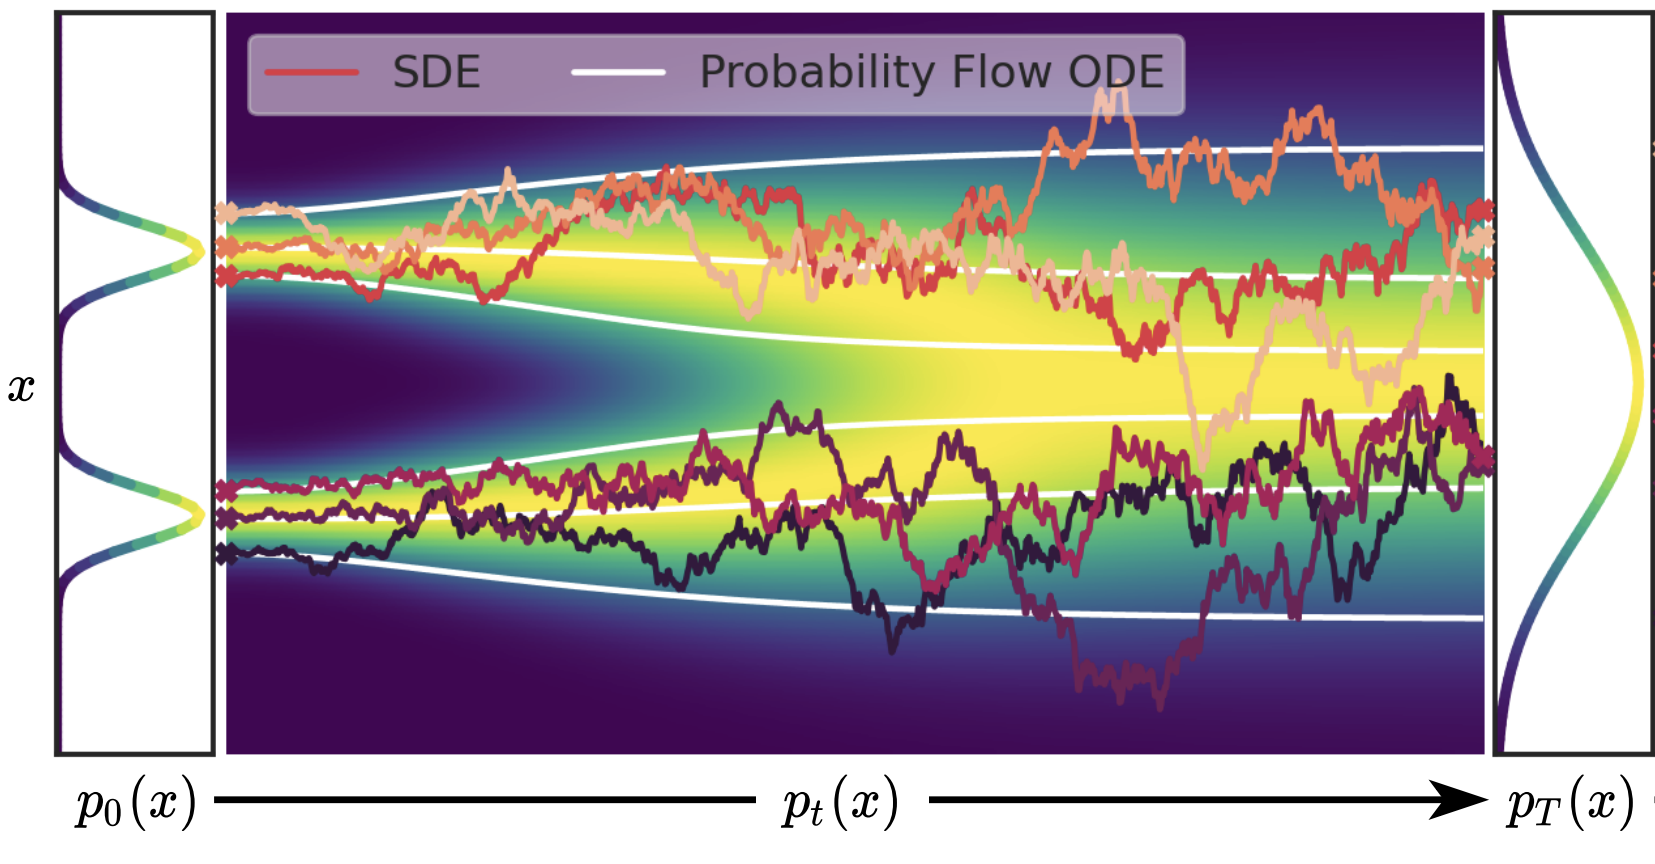
\includegraphics[width=0.75\linewidth]{figs/probability_flow}
	\end{figure}
\end{frame}
%=======
\begin{frame}{Probability Flow ODE}
	\myfootnotewithlink{https://arxiv.org/abs/2011.13456}{Song Y., et al. Score-Based Generative Modeling through Stochastic Differential Equations, 2020}
	\vspace{-0.3cm}
	\begin{block}{Theorem}
		Suppose the SDE $d\bx = \bff(\bx, t) dt + g(t) d \bw$ induces the probability path $p_t(\bx)$ with $p_t(\bx) > 0$.
		Then, there exists an ODE with the same probability path $p_t(\bx)$, given by
		\vspace{-0.3cm}
		\[
			d\bx = \bv(\bx, t) dt = \left(\bff(\bx, t) -\frac{1}{2} g^2(t) \frac{\partial}{\partial \bx} \log p_t(\bx) \right) dt
		\]
		\vspace{-0.7cm}
	\end{block}
	\begin{block}{Proof}
 		\vspace{-0.7cm}
 		{\small
 		\begin{multline*}
 			\frac{\partial p_t(\bx)}{\partial t} = \tr\left( - \frac{\partial}{\partial \bx} \bigl[ \bff(\bx, t) p_t(\bx)\bigr] + \frac{1}{2} g^2(t) \frac{\partial^2 p_t(\bx)}{\partial \bx^2} \right) 
			\nextonslide{= \\ = \tr\left( - \frac{\partial}{\partial \bx} \left[ \bff(\bx, t) p_t(\bx) - \frac{1}{2} g^2(t) {\color{violet}\frac{\partial p_t(\bx)}{\partial \bx}} \right]  \right)}
			\nextonslide{ = \\ =  \tr\left( - \frac{\partial}{\partial \bx} \left[ \bff(\bx, t) p_t(\bx) - \frac{1}{2} g^2(t) {\color{violet}p_t(\bx) \frac{\partial}{\partial \bx} \log p_t(\bx)} \right]  \right)}
			\nextonslide{= \\ =  \tr\left( - \frac{\partial}{\partial \bx} \left[ \left( {\color{teal}\bff(\bx, t) - \frac{1}{2} g^2(t) \frac{\partial}{\partial \bx} \log p_t(\bx)}\right) p_t(\bx) \right]  \right)}
 		\end{multline*}
 		}
 	\end{block}
\end{frame}
%=======
\begin{frame}{Probability Flow ODE}
	\myfootnotewithlink{https://arxiv.org/abs/2011.13456}{Song Y., et al. Score-Based Generative Modeling through Stochastic Differential Equations, 2020}
	\begin{block}{Proof (Continued)}
 		\vspace{-0.7cm}
 		\begin{multline*}
 			\frac{\partial p_t(\bx)}{\partial t} =  \tr\left( - \frac{\partial}{\partial \bx} \left[ \left( {\color{teal}\bff(\bx, t) - \frac{1}{2} g^2(t) \frac{\partial}{\partial \bx}\log p_t(\bx)}\right) p_t(\bx) \right]  \right) 
			\nextonslide{=\\ =  \tr\left( - \frac{\partial}{\partial \bx} \left[ {\color{teal}\bv(\bx, t)} p_t(\bx) \right]  \right) = -  \diver\left(\bv(\bx, t) p_t(\bx)\right)}
 		\end{multline*}
		\eqpause
		\[
			\bv(\bx, t) = \bff(\bx, t) -\frac{1}{2} g^2(t) \frac{\partial}{\partial \bx} \log p_t(\bx); \quad \tilde{g}(t) = 0
		\]
	 	\[
	 		d \bx = \bv(\bx, t) dt + 0 \cdot d \bw = \left(\bff(\bx, t) -\frac{1}{2} g^2(t) \frac{\partial}{\partial \bx} \log p_t(\bx) \right) dt
	 	\]
		\[
			\frac{\partial p_t(\bx)}{\partial t} = - \diver(\bv(\bx, t) p_t(\bx)) + \frac{1}{2}\tilde{g}^2(t) \Delta_{\bx}p_t(\bx)
		\]
 	\end{block}
\end{frame}
%=======
\begin{frame}{Probability Flow ODE}
	\myfootnotewithlink{https://arxiv.org/abs/2011.13456}{Song Y., et al. Score-Based Generative Modeling through Stochastic Differential Equations, 2020}
	\vspace{-0.3cm}
	\begin{align*}
		d\bx &= \bff(\bx, t) dt + g(t) d \bw \;\; - \text{SDE} \\
		d\bx &= \bv(\bx, t) dt  \;\; - \text{Probability Flow ODE}
	\end{align*}
	\vspace{-0.5cm}
	\[
		\bv(\bx, t) = \bff(\bx, t) -\frac{1}{2} g^2(t) \frac{\partial}{\partial \bx} \log p_t(\bx)
	\]
	\eqpause
	\vspace{-0.3cm}
	\begin{itemize}
		\item $\bs(\bx, t) = \frac{\partial}{\partial \bx} \log p_t(\bx)$ is the continuous-time score function.
		\eqpause
		\item The ODE produces more stable trajectories.
	\end{itemize}
	\vspace{-0.3cm}
	\begin{figure}
		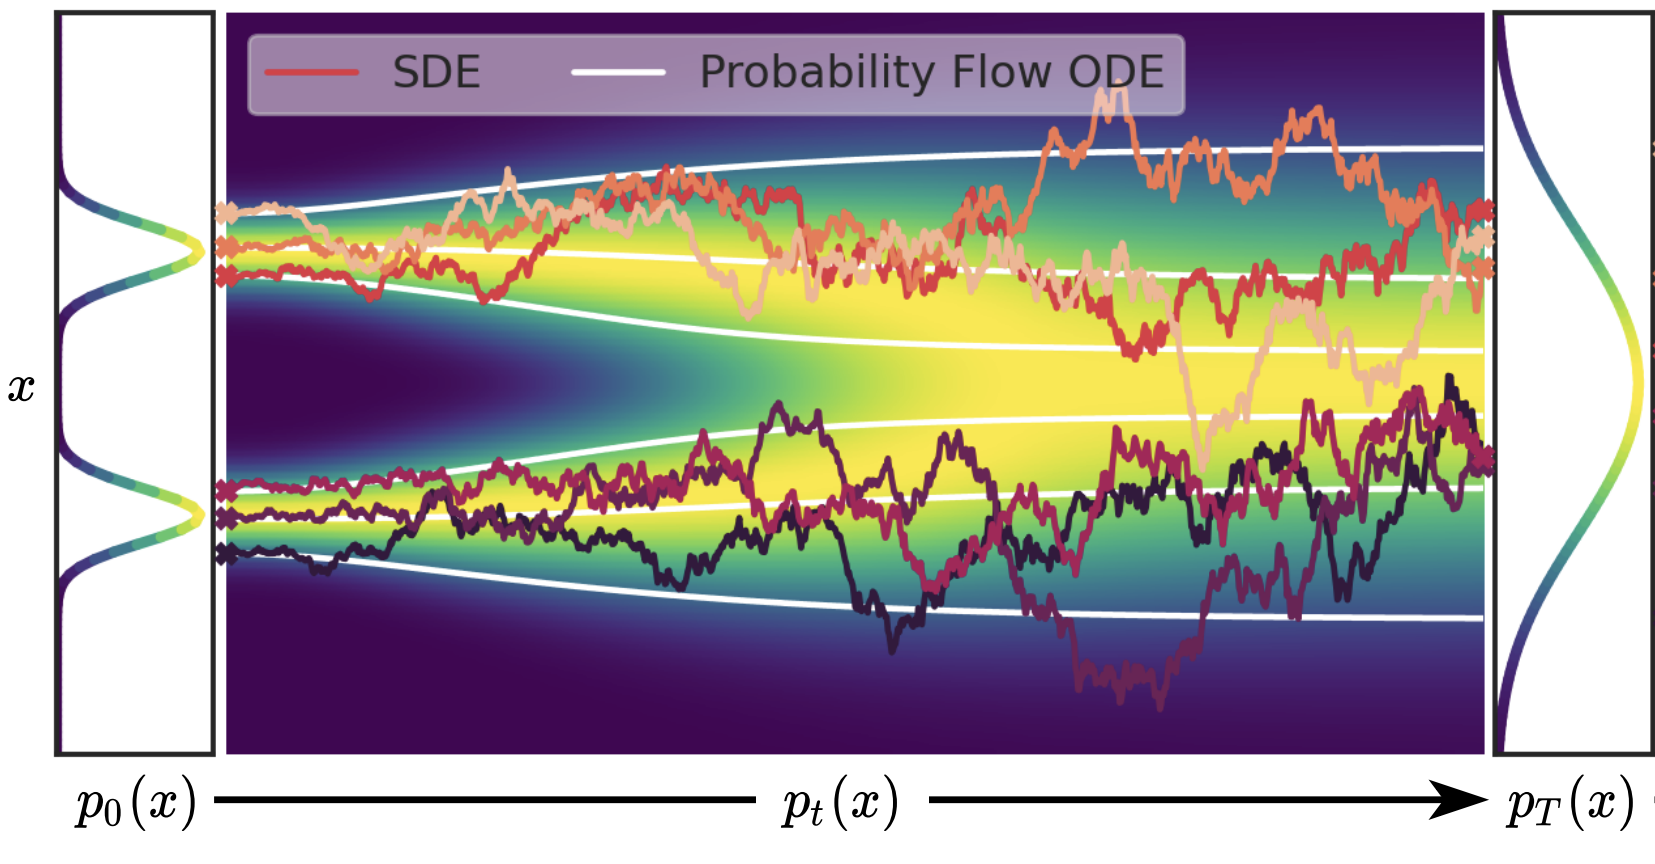
\includegraphics[width=0.75\linewidth]{figs/probability_flow}
	\end{figure}
\end{frame}
%=======
\begin{frame}{Why convert SDEs to PF-ODEs? (1) Efficient Sampling}
	\myfootnotewithlink{https://arxiv.org/abs/2206.00364}{Karras T., et al. Elucidating the Design Space of Diffusion-Based Generative Models, 2022}
	\begin{itemize}
		\item Brownian increments scale as $d\bw \sim \sqrt{dt}$ — SDE trajectories are nowhere differentiable.
		\item \SDESolve (Euler–Maruyama): local error $\cO(\sqrt{\Delta t})$.
		\item Higher-order SDE schemes need Lévy areas $\Rightarrow$ impractical in high dimensions.
	\end{itemize}
	\eqpause
	\begin{block}{PF-ODE drift $\bv(\bx, t) = \bff(\bx, t) - \frac{1}{2} g^2(t) \bs(\bx, t)$ is smooth}
		\begin{itemize}
			\item Euler: $\cO(\Delta t)$, \quad Heun: $\cO(\Delta t^2)$, \quad RK4: $\cO(\Delta t^4)$.
			\item Adaptive step-size control is standard for \ODESolve.
		\end{itemize}
	\end{block}
	\eqpause
	\begin{itemize}
		\item In practice: $100$--$1000$ \SDESolve steps $\to$ $20$--$50$ \ODESolve steps.
		\item Caveat: SDE sampling can still win at high NFE — injected noise corrects accumulated error.
	\end{itemize}
\end{frame}
%=======
\begin{frame}{Why convert SDEs to PF-ODEs? (2) Deterministic Generation}
	\myfootnotewithlink{https://arxiv.org/abs/1806.07366}{Chen R. T. Q., et al. Neural Ordinary Differential Equations, 2018}
	\begin{itemize}
		\item The PF-ODE defines a deterministic, invertible map $\bx(0) \leftrightarrow \bx(T)$.
		\item Each terminal $\bx(T)$ produces a unique trajectory back to data space.
	\end{itemize}
	\eqpause
	\begin{block}{Exact log-likelihood (instantaneous change of variables)}
		\vspace{-0.3cm}
		\[
			\log p_0(\bx(0)) = \log p_T(\bx(T)) + \int_0^T \tr\left(\frac{\partial \bv(\bx(t), t)}{\partial \bx(t)}\right) dt
		\]
	\end{block}
	\eqpause
	\begin{itemize}
		\item Connects PF-ODE to continuous normalizing flows.
		\item Invertibility enables image $\to$ latent $\to$ edited image workflows.
		\item Smooth interpolation in latent space between two samples.
	\end{itemize}
\end{frame}
%=======
\begin{frame}{Sampling: Reverse SDE vs PF-ODE}
	\myfootnotewithlink{https://arxiv.org/abs/2011.13456}{Song Y., et al. Score-Based Generative Modeling through Stochastic Differential Equations, 2020}
	Same trained score $\bs_{\btheta}(\bx, t)$; only the discretization changes (reverse SDE derived in the next section).
	\eqpause
	\begin{block}{Sampling (Reverse SDE, Euler--Maruyama)}
		\begin{enumerate}
			\item Sample $\bx_T \sim \cN(0, \bI)$.
			\item Initialize step $\Delta t = T / K$.
			\item Denoise:
			\vspace{-0.2cm}
			\[
				\bx_{t - \Delta t} = \bx_t - \Bigl[\bff(\bx_t, t) - {\color{violet}g^2(t)}\, \bs_{\btheta}(\bx_t, t)\Bigr] \Delta t \, {\color{violet}+ \, g(t)\sqrt{\Delta t} \cdot \bepsilon}, \;\; \bepsilon \sim \cN(0, \bI)
			\]
			\vspace{-0.5cm}
		\end{enumerate}
	\end{block}
	\eqpause
	\begin{block}{Sampling (PF-ODE: Euler / Heun / RK4)}
		\begin{enumerate}
			\item Sample $\bx_T \sim \cN(0, \bI)$.
			\item Initialize step $\Delta t = T / K$ \,(with $K \ll$ SDE case).
			\item Denoise:
			\vspace{-0.2cm}
			\[
				\bx_{t - \Delta t} = \bx_t - \Bigl[\bff(\bx_t, t) - {\color{teal}\tfrac{1}{2}\, g^2(t)}\, \bs_{\btheta}(\bx_t, t)\Bigr] \Delta t \;\; {\color{teal}(\text{no noise injection})}
			\]
			\vspace{-0.5cm}
		\end{enumerate}
	\end{block}
\end{frame}
%=======
\section{Reverse SDE}
%=======
\begin{frame}{Reverse SDE}
	\myfootnotewithlink{https://arxiv.org/abs/2011.13456}{Song Y., et al. Score-Based Generative Modeling through Stochastic Differential Equations, 2020}
	\vspace{-0.3cm}
	\[
		d\bx = \bv(\bx, t) dt,\qquad \bx(t + dt) = \bx(t) + \bv(\bx, t) dt
	\]
	Here $dt$ can be $>0$ or $<0$.
	\eqpause
	\begin{block}{Reverse ODE}
		Let $\tau = 1 - t$ ($d\tau = -dt$).
		\vspace{-0.3cm}
		\[
			d\bx = - \bv(\bx, 1 - \tau) d\tau
		\]
	\end{block}
	\eqpause
	\vspace{-0.5cm}
	\begin{itemize}
		\item How do we reverse the SDE $d\bx = \bff(\bx, t) dt + g(t) d \bw$? 
		\item The Wiener process introduces randomness that must be reversed.
	\end{itemize}
	\eqpause
	\vspace{-0.3cm}
	\begin{block}{Theorem}
		There exists a reverse SDE for $d\bx = \bff(\bx, t) dt + g(t) d \bw$ (assume $p_t(\bx) > 0$), given by:
		\vspace{-0.3cm}
		\[
			d\bx = \left(\bff(\bx, t) - g^2(t) \frac{\partial}{\partial \bx}\log p_t(\bx)\right) dt + g(t) d \bar{\bw}
		\]
		\vspace{-0.5cm}\\
		where $dt<0$ and $\bar{\bw}$ is a reverse-time Wiener process.
	\end{block}
\end{frame}
%=======
\begin{frame}{Reverse SDE}
	\myfootnotewithlink{https://arxiv.org/abs/2011.13456}{Song Y., et al. Score-Based Generative Modeling through Stochastic Differential Equations, 2020}
	\begin{block}{Theorem}
		There exists a reverse SDE for $d\bx = \bff(\bx, t) dt + g(t) d \bw$ (assume $p_t(\bx) > 0$), given by:
		\vspace{-0.3cm}
		\[
			d\bx = \left(\bff(\bx, t) {\color{violet}- g^2(t) \frac{\partial}{\partial \bx}\log p_t(\bx)}\right) dt + g(t) d \bar{\bw}
		\]
		\vspace{-0.5cm}\\
		where $dt<0$ and $\bar{\bw}(t)$ is a reverse-time Wiener process.
	\end{block}
	\eqpause
	\begin{itemize}
		\item Here the score function appears: $\bs(\bx, t) = \frac{\partial}{\partial \bx} \log p_t(\bx)$.
		\item Since $\bv(\bx, t) = \bff(\bx, t) - \frac{1}{2} g^2(t) \bs(\bx, t)$ (PF-ODE), the reverse drift equals $\bff - g^2 \bs = \bv - \frac{1}{2} g^2 \bs$.
	\end{itemize}
	\eqpause
	\begin{block}{Proof Sketch}
		\begin{itemize}
			\item Convert the initial SDE to a probability flow ODE.
			\item Reverse the probability flow ODE.
			\item Convert the reversed probability flow ODE back to an SDE.
		\end{itemize}
	\end{block}
\end{frame}
%=======
\begin{frame}{Proof of Reverse SDE}
	\myfootnotewithlink{https://arxiv.org/abs/2011.13456}{Song Y., et al. Score-Based Generative Modeling through Stochastic Differential Equations, 2020}	
	\vspace{-0.3cm}
	\begin{itemize}
			\item Convert the initial SDE to a probability flow ODE:
			\vspace{-0.1cm}
			{\footnotesize
			\begin{align*}
				d\bx &= \bff(\bx, t) dt + g(t) d \bw \\
				d\bx &= \left(\bff(\bx, t) -\frac{1}{2} g^2(t) \frac{\partial}{\partial \bx} \log p_t(\bx) \right) dt
			\end{align*}
			}
			\vspace{-0.5cm}
			\eqpause
			\item Reverse the probability flow ODE:
			\vspace{-0.1cm}
			{\footnotesize
			\begin{align*}
				d\bx &= \left(\bff(\bx, t) -\frac{1}{2} g^2(t) \frac{\partial}{\partial \bx} \log p_t(\bx) \right) dt \\
				d\bx &= \left(-\bff(\bx, 1 - \tau) + \frac{1}{2} g^2(1 - \tau) \frac{\partial}{\partial \bx} \log p_{1 - \tau}(\bx) \right) d\tau
			\end{align*}
			}
			\vspace{-0.5cm}
			\eqpause
			\item Convert the reversed probability flow ODE back to an SDE:
			\vspace{-0.1cm}
			{\footnotesize
			\begin{align*}
				d\bx &= \left(-\bff(\bx, 1 - \tau) + \frac{1}{2} g^2(1 - \tau) \frac{\partial}{\partial \bx} \log p_{1 - \tau}(\bx) \right) d \tau \\
				d\bx &= \left(-\bff(\bx, 1 - \tau) + g^2(1 - \tau) \frac{\partial}{\partial \bx} \log p_{1 - \tau}(\bx) \right) d \tau + g(1-\tau)d\bw
			\end{align*}
			}
			Here $\bw(\tau)$ is a Wiener process in forward $\tau$-time.
		\end{itemize}
\end{frame}
%=======
\begin{frame}{Reverse SDE}
	\myfootnotewithlink{https://arxiv.org/abs/2011.13456}{Song Y., et al. Score-Based Generative Modeling through Stochastic Differential Equations, 2020}
	\begin{block}{Theorem}
		There exists a reverse SDE for $d\bx = \bff(\bx, t) dt + g(t) d \bw$ (assume $p_t(\bx) > 0$), given by:
		\vspace{-0.3cm}
		\[
			d\bx = \left(\bff(\bx, t) {\color{violet}- g^2(t) \frac{\partial}{\partial \bx}\log p_t(\bx)}\right) dt + g(t) d \bar{\bw}
		\]
		\vspace{-0.5cm}\\
		where $dt<0$ and $\bar{\bw}(t)$ is a reverse-time Wiener process.
	\end{block}
	\begin{block}{Proof (Continued)}
		\vspace{-0.7cm}
		\[
			d\bx = \left(-\bff(\bx, 1 - \tau) + g^2(1 - \tau) \frac{\partial}{\partial \bx} \log p_{1 - \tau}(\bx) \right)d\tau + g(1 - \tau) d \bw
		\]
		\eqpause
		\[
			d\bx = \left(\bff(\bx, t) - g^2(t) \frac{\partial}{\partial \bx}\log p_t(\bx)\right)dt + g(t) d\bar{\bw}
		\]
		Here $d\tau > 0$, $dt < 0$, and $\bar{\bw}$ is reverse-time Wiener process.
	\end{block}
\end{frame}
%=======
\begin{frame}{Reverse SDE}
	\myfootnotewithlink{https://arxiv.org/abs/2011.13456}{Song Y., et al. Score-Based Generative Modeling through Stochastic Differential Equations, 2020}
	\[
		d\bx = \bff(\bx, t) dt + g(t) d \bw
	\]
	\vspace{-0.3cm}
	\[
		\bv(\bx, t) = \bff(\bx, t) - \frac{1}{2} g^2(t) \bs(\bx, t), \quad \text{where} \quad \bs(\bx, t) = \nabla_{\bx} \log p_t(\bx)
	\]
	\vspace{-0.3cm}
	\begin{align*}
		d\bx &= \bv(\bx, t) dt \;\; - \textbf{Probability Flow ODE} \\
		d\bx &= \bigl({\color{violet}\bv(\bx, t) - \frac{1}{2} g^2(t) \bs(\bx, t)}\bigr) dt + g(t) d \bar{\bw} \;\; - \textbf{Reverse SDE}
	\end{align*}
	\eqpause
	\vspace{-0.7cm}
	\begin{figure}
		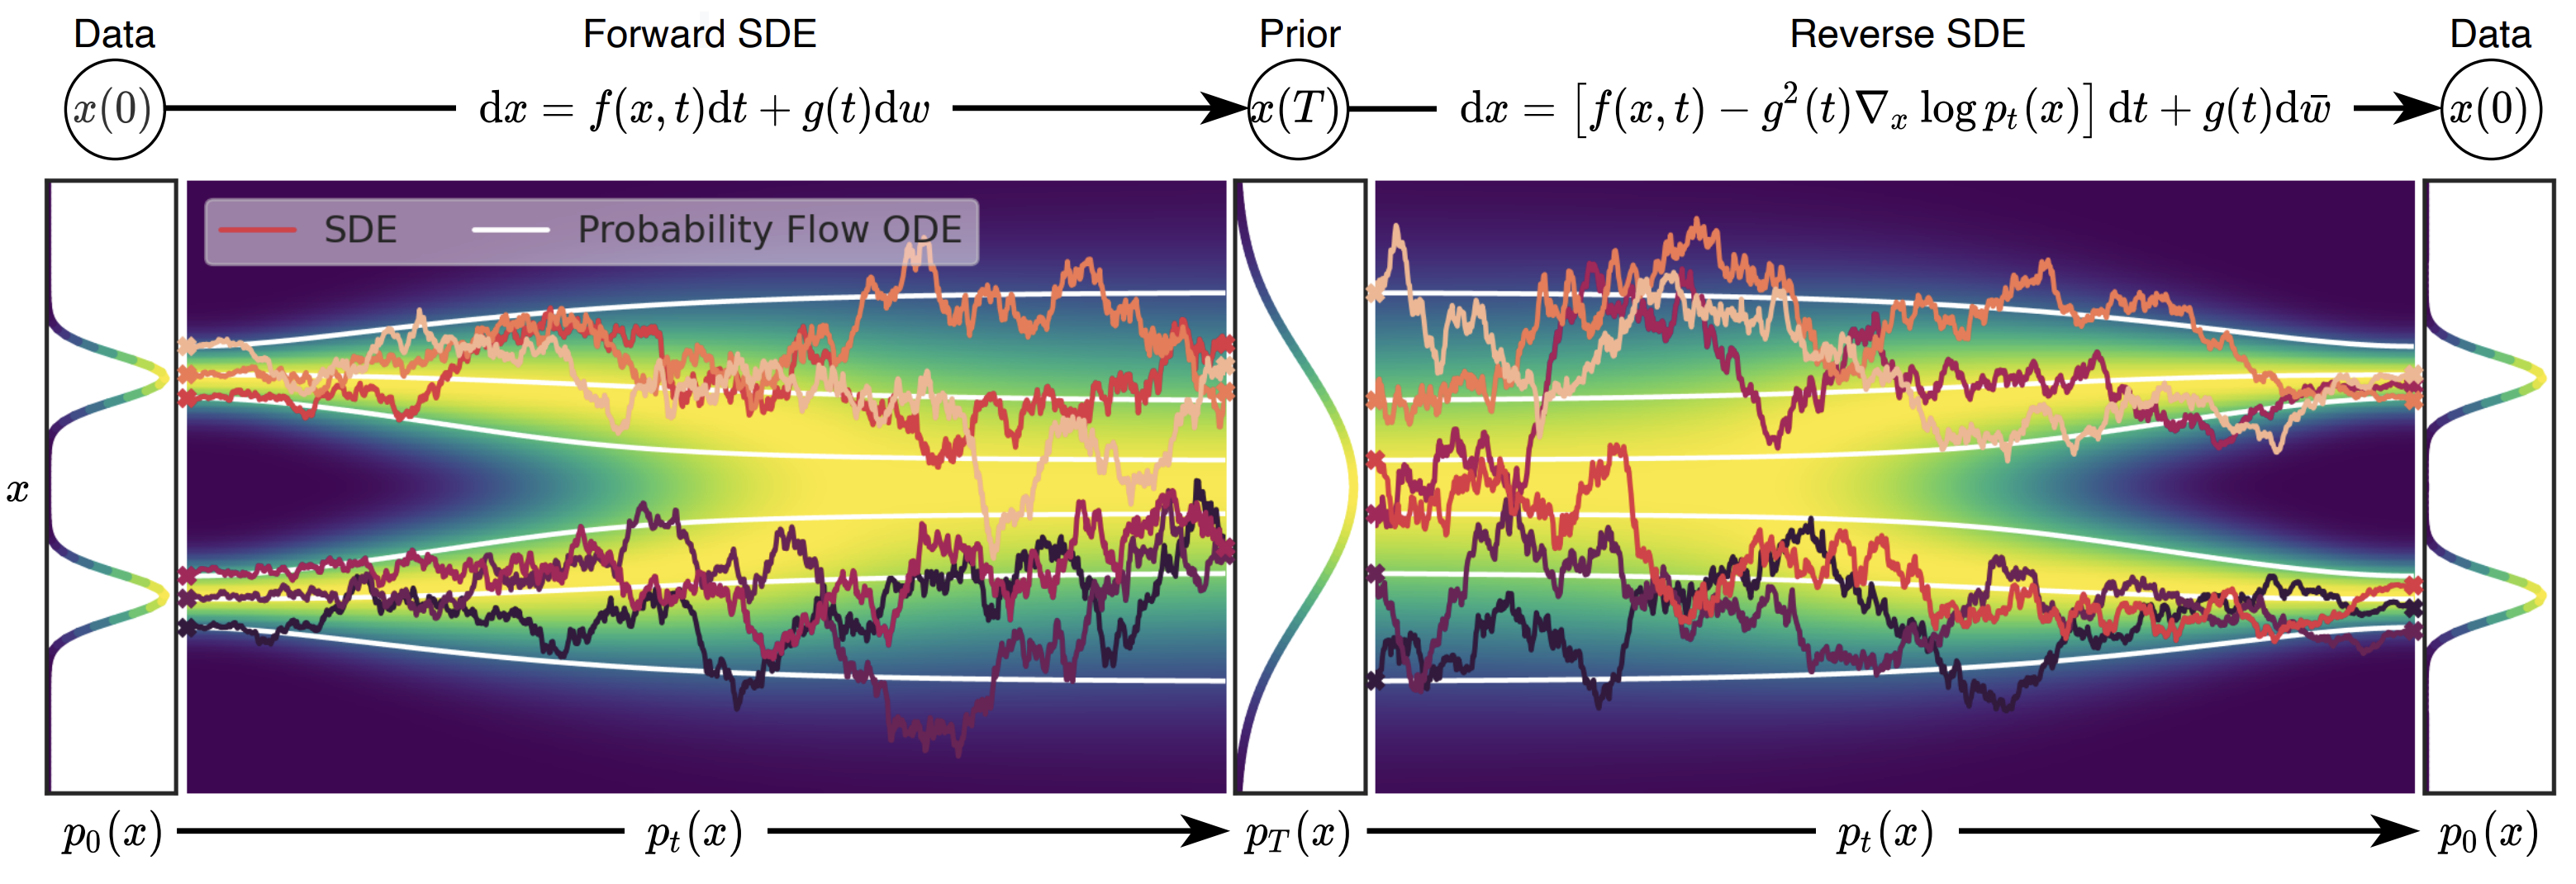
\includegraphics[width=1.0\linewidth]{figs/sde}
	\end{figure}
\end{frame}
%=======
\begin{frame}{Score Matching SDE}
	\myfootnotewithlink{https://arxiv.org/abs/2011.13456}{Song Y., et al. Score-Based Generative Modeling through Stochastic Differential Equations, 2020}
	\vspace{-0.3cm}
	\[
		\bx(t) = \bx(t - dt) + \sqrt{\frac{ d [\sigma^2(t)]}{dt}} \cdot d \bw
	\]
    \eqpause
	\vspace{-0.5cm}
	\begin{block}{Variance Exploding SDE}
		\vspace{-0.3cm}
		\[
			d \bx = \sqrt{\frac{ d [\sigma^2(t)]}{dt}} \cdot d \bw
		\]
		$\sigma(t)$ is a monotonically increasing function.
	\end{block}
    \eqpause
	\vspace{-0.7cm}
	\[
		d\bx = \bff(\bx, t) dt + g(t) d \bw, \quad \bff(\bx, t) = 0, \quad g(t) = \sqrt{\frac{ d [\sigma^2(t)]}{dt}} 
	\]
    \eqpause
	\vspace{-0.5cm}
	\begin{align*}
		d\bx &= \left(-\frac{1}{2} \frac{ d [\sigma^2(t)]}{dt} \frac{\partial}{\partial \bx} \log p_t(\bx) \right) dt \qquad\quad\, \text{(probability flow ODE)} \\
		d\bx &= \left(- \frac{ d [\sigma^2(t)]}{dt} \frac{\partial}{\partial \bx}\log p_t(\bx)\right) dt + \sqrt{\frac{ d [\sigma^2(t)]}{dt}}  d \bar{\bw} \ \ \text{(reverse SDE)}
	\end{align*}
\end{frame}
%=======
\begin{frame}{Diffusion SDE}
	\myfootnotewithlink{https://arxiv.org/abs/2011.13456}{Song Y., et al. Score-Based Generative Modeling through Stochastic Differential Equations, 2020}
	\begin{block}{Variance Preserving SDE}
		\vspace{-0.3cm}
		\[
			d \bx = - \frac{1}{2} \beta(t) \bx(t) dt + \sqrt{\beta(t)} \cdot d \bw
		\]
		\[
			\bff(\bx, t) = - \frac{1}{2} \beta(t) \bx(t) , \quad g(t) = \sqrt{\beta(t)} 
		\]
	\end{block}
	Variance is preserved as long as $\bx(0)$ has unit variance.
    \eqpause
	\begin{align*}
		d\bx &= \left(- \frac{1}{2} \beta(t) \bx(t) - \frac{1}{2} \beta(t) \frac{\partial}{\partial \bx} \log p_t(\bx) \right) dt \quad\quad \text{(probability flow ODE)} \\
		d\bx &= \left(- \frac{1}{2} \beta(t) \bx(t) - \beta(t) \frac{\partial}{\partial \bx} \log p_t(\bx)\right) dt + \sqrt{\beta(t)} d \bar{\bw}\ \ \text{(reverse SDE)}
	\end{align*}
\end{frame}
%=======
\section{Score-Based Generative Models Through SDEs}
%=======
\begin{frame}{Score-Based Generative Models Through SDEs}
    \myfootnotewithlink{https://arxiv.org/abs/2011.13456}{Song Y., et al. Score-Based Generative Modeling through Stochastic Differential Equations, 2020}
	\begin{block}{Discrete-Time Objective}
		\vspace{-0.3cm}
		\[
			\bbE_{\pd(\bx_0)} \bbE_{t \sim U\{1, T\}} \bbE_{q(\bx_t | \bx_0)}\bigl\| \bs_{\btheta, t}(\bx_t) - \nabla_{\bx_t} \log q(\bx_t | \bx_0) \bigr\|^2_2 
		\]
		\vspace{-0.5cm}
	\end{block}
	Is it possible to train score-based diffusion models in continuous time?
    \eqpause
	\begin{block}{Continuous-Time Objective}
		\vspace{-0.7cm}
		\[
			\bbE_{\pd(\bx(0))} \bbE_{t \sim U[0, 1]} \bbE_{q(\bx(t) | \bx(0))}\bigl\| \bs_{\btheta}(\bx(t), t) - {\color{teal}\nabla_{\bx(t)} \log q(\bx(t) | \bx(0))} \bigr\|^2_2 
		\]
		\vspace{-0.7cm}
	\end{block}
    \eqpause
	\vspace{-0.4cm}
	\begin{figure}
		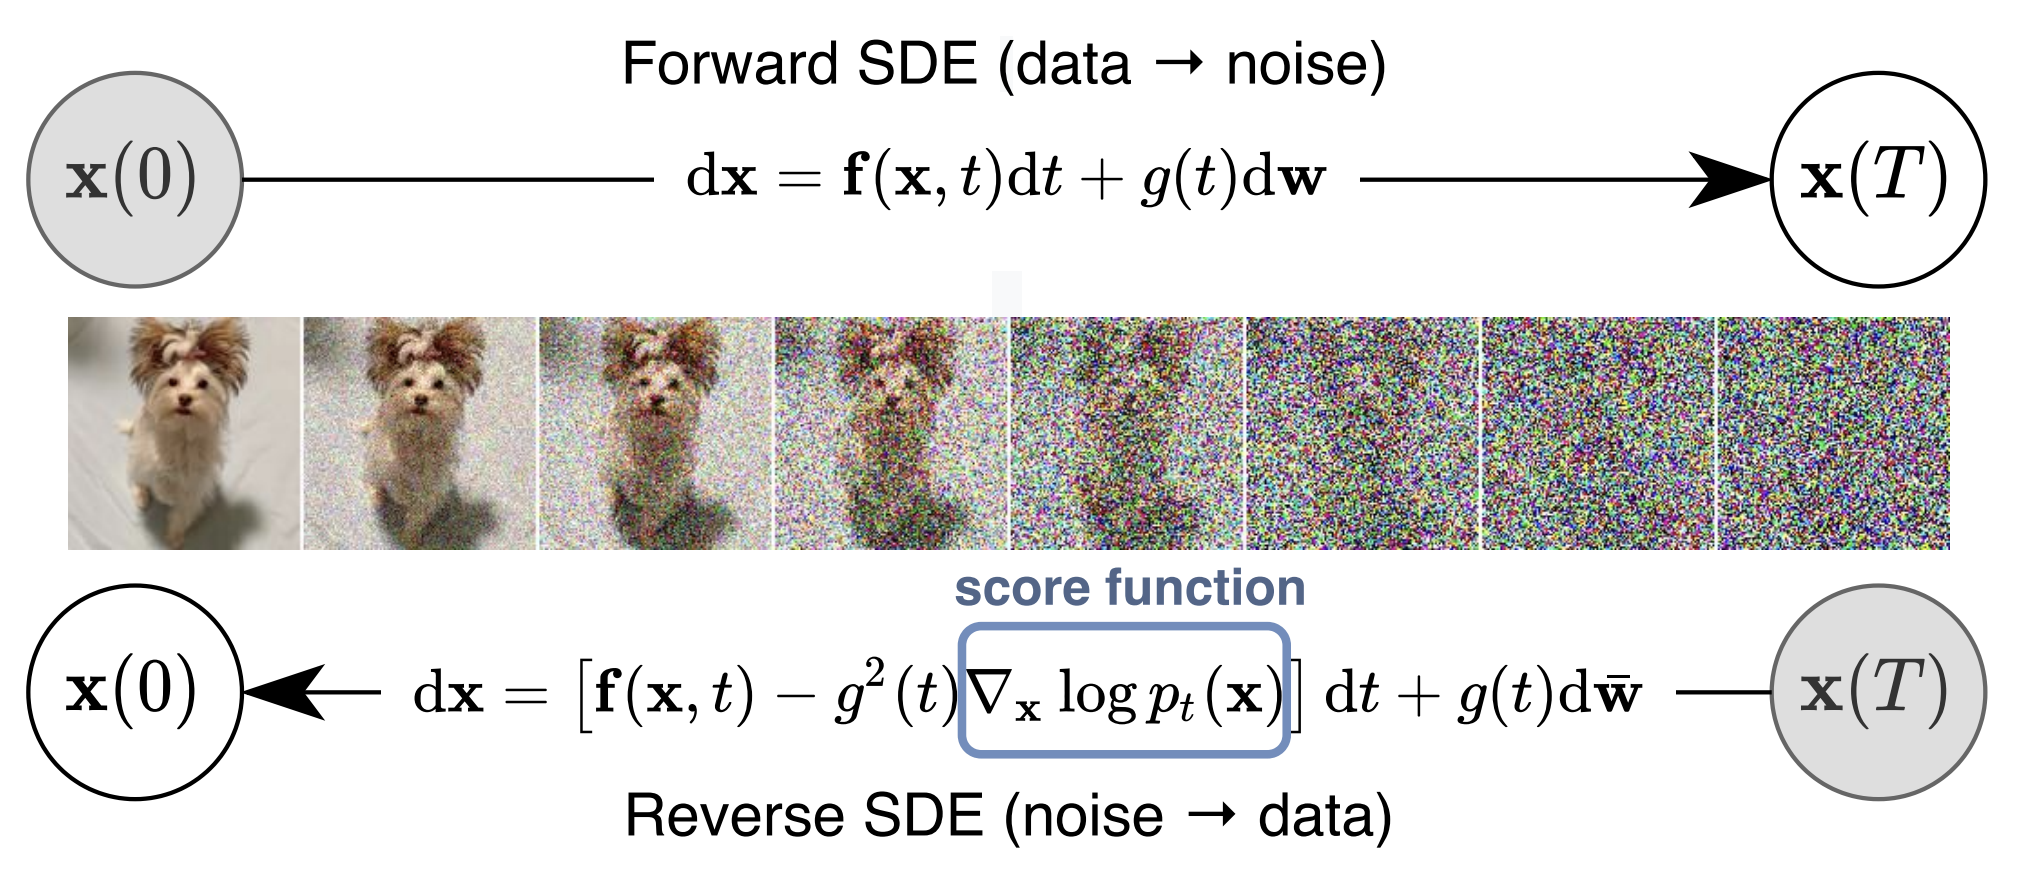
\includegraphics[width=0.75\linewidth]{figs/sbgm}
	\end{figure}
\end{frame}
%=======
\begin{frame}{Generative Models Taxonomy}
	\renderTaxonomy{sde}
\end{frame}
%=======
\begin{frame}{Score-Based Generative Models Through SDEs}
	\myfootnotewithlink{https://users.aalto.fi/~asolin/sde-book/sde-book.pdf}{Särkkä S., Solin A. Applied stochastic differential equations, 2019}
	\vspace{-0.3cm}
	\begin{block}{Continuous-Time Objective}
		\vspace{-0.7cm}
		\[
			\bbE_{\pd(\bx(0))} \bbE_{t \sim U[0, 1]} \bbE_{q(\bx(t) | \bx(0))}\bigl\| \bs_{\btheta}(\bx(t), t) - {\color{teal}\nabla_{\bx(t)} \log q(\bx(t) | \bx(0))} \bigr\|^2_2 
		\]
		\vspace{-0.7cm}
	\end{block}
    \eqpause
	\[
		q(\bx(t) | \bx(0)) = \cN\Bigl(\bmu(\bx(0), t), \sigma^2(t) \cdot \bI \Bigr) 
	\]
	\[
		\nabla_{\bx(t)} \log q(\bx(t) | \bx(0)) = - \frac{1}{\sigma^2(t)} (\bx(t) - \bmu)
	\]
	\textbf{Note:} Normality holds for $\bff(\bx, t)$ affine in $\bx$ ($\bff(\bx, t) = f(t) \bx$).
    \eqpause
	\[
		d \bx = \sqrt{\frac{ d [\sigma^2(t)]}{dt}} \cdot d \bw \ \ \mbox{(Variance Exploding SDE)}
	\]
	\vspace{-0.3cm}
	\[
		d \bx = - \frac{1}{2} \beta(t) \bx(t) dt + \sqrt{\beta(t)} \cdot d \bw \ \ \mbox{(Variance Preserving SDE)}
	\]
	Is it possible to explicitly derive $\bmu(\bx(0), t)$ and $\sigma^2(t)$ for VE-SDE and VP-SDE?
\end{frame}
%=======
\begin{frame}{Score-Based Generative Models Through SDEs}
	\myfootnotewithlink{https://users.aalto.fi/~asolin/sde-book/sde-book.pdf}{Särkkä S., Solin A. Applied stochastic differential equations, 2019}
	\[
		q(\bx(t) | \bx(0)) = \cN\Bigl(\bmu(\bx(0), t), \sigma^2(t) \cdot \bI\Bigr)
	\]
	\vspace{-0.5cm}
	\begin{block}{Theorem}
		The moments of the SDE $d\bx = f(t) \bx dt + g(t) d \bw$ satisfy:
		\[
			\frac{d \bmu(\bx(0), t)}{dt} = f(t) \bmu(\bx(0), t)
		\]
		\[
			\frac{d \sigma^2(t)}{dt} = 2 f(t) \sigma^2(t) + g^2(t)
		\]
	\end{block}
    \eqpause
	\begin{block}{Proof}
		\vspace{-0.7cm}
		\begin{align*}
			\bbE\left[{\color{violet}d\bx} | \bx(0) \right] &= \bbE\left[{\color{violet}f(t) \bx dt} | \bx(0) \right] + \bbE\left[{\color{violet}g(t) d \bw} | \bx(0) \right]
			\nextonslide{\\ &= f(t) \bbE\left[\bx | \bx(0) \right] dt + g(t) \bbE\left[d \bw | \bx(0) \right]}
			\nextonslide{\\ &= f(t) \bmu(\bx(0), t) dt}
		\end{align*}
	\end{block}
\end{frame}
%=======
\begin{frame}{Score-Based Generative Models Through SDEs}
	\myfootnotewithlink{https://users.aalto.fi/~asolin/sde-book/sde-book.pdf}{Särkkä S., Solin A. Applied stochastic differential equations, 2019}
	\begin{block}{Theorem}
		\vspace{-0.3cm}
		\[
			\frac{d \bmu(\bx(0), t)}{dt} = f(t) \bmu(\bx(0), t)
		\]
		\vspace{-0.5cm}
	\end{block}
    \eqpause
	\begin{block}{Proof (Continued)}
		\vspace{-0.3cm}
		\[
			\bbE\left[d\bx | \bx(0) \right] = f(t) \bmu(\bx(0), t) dt
		\]
        \eqpause
		\[
			\frac{d \bbE\left[\bx(t) | \bx(0) \right]}{dt} = \frac{d \bmu(\bx(0), t)}{dt} = f(t) \bmu(\bx(0), t) 
		\]
	\end{block}
    \eqpause
	\vspace{-0.3cm}
	\begin{block}{Examples}
		\vspace{-0.5cm}
		\[
			\textbf{NCSN:}\quad	f(t) = 0 \quad \Rightarrow \quad \bmu = \bx(0)
		\]
        \eqpause
		\vspace{-0.5cm}
		\[
			\textbf{DDPM:}\quad f(t) = - \frac{1}{2} \beta(t)\;\;   \Rightarrow\quad \frac{d \bmu}{dt} = - \frac{1}{2} \beta(t) \bmu
		\]
        \eqpause
		\vspace{-0.3cm}
		\[
			\bmu = \bx(0) \exp\left(- \frac{1}{2} \int_0^t \beta(s)ds\right)
		\]
	\end{block}
\end{frame}
%=======
\begin{frame}{Score-Based Generative Models Through SDEs}
	\myfootnotewithlink{https://arxiv.org/abs/2011.13456}{Song Y., et al. Score-Based Generative Modeling through Stochastic Differential Equations, 2020}
	\begin{block}{Training}
		\begin{enumerate}
			\item Sample $\bx(0) \sim \pd(\bx)$, $t \sim U[0, 1]$.
			\item Sample $\bx(t) \sim q(\bx(t) | \bx(0))$.
			\item Compute loss $\cL = \bigl\| \bs_{\btheta}(\bx(t), t) - {\color{teal}\nabla_{\bx(t)} \log q(\bx(t) | \bx(0))} \bigr\|^2_2$.
		\end{enumerate}
	\end{block}
	\[
		q(\bx(t) | \bx(0)) = \cN\Bigl(\bmu(\bx(0), t), \sigma^2(t) \cdot \bI\Bigr)
	\]
    \eqpause
	\vspace{-0.5cm}
	\begin{block}{NCSN}
		\vspace{-0.3cm}
		\[
			q(\bx(t) | \bx(0)) = \cN\left(\bx(0), \left[\sigma^2(t) - \sigma^2(0)\right] \cdot \bI\right)
		\]
		\vspace{-0.5cm}
	\end{block}
    \eqpause
	\begin{block}{DDPM}
		\vspace{-0.5cm}
		\[
			q(\bx(t) | \bx(0)) = \cN\left(\bx(0) e^{-\frac{1}{2} \int_0^t\beta(s)ds}, \left(1 - e^{- \int_0^t\beta(s)ds}\right) \cdot \bI\right)
		\]
		\vspace{-0.5cm}
	\end{block}
	Here we omit the derivations of the variance.
	
\end{frame}
%=======
\begin{frame}{Score-Based Generative Models Through SDEs}
	\myfootnotewithlink{https://arxiv.org/abs/2011.13456}{Song Y., et al. Score-Based Generative Modeling through Stochastic Differential Equations, 2020}
	\begin{block}{Sampling}
		\begin{enumerate}
			\item Sample $\bx(1) \sim \cN(0, \bI)$.
			\item Solve the reverse SDE using numerical solvers (\SDESolve).
		\end{enumerate}
		\begin{figure}
			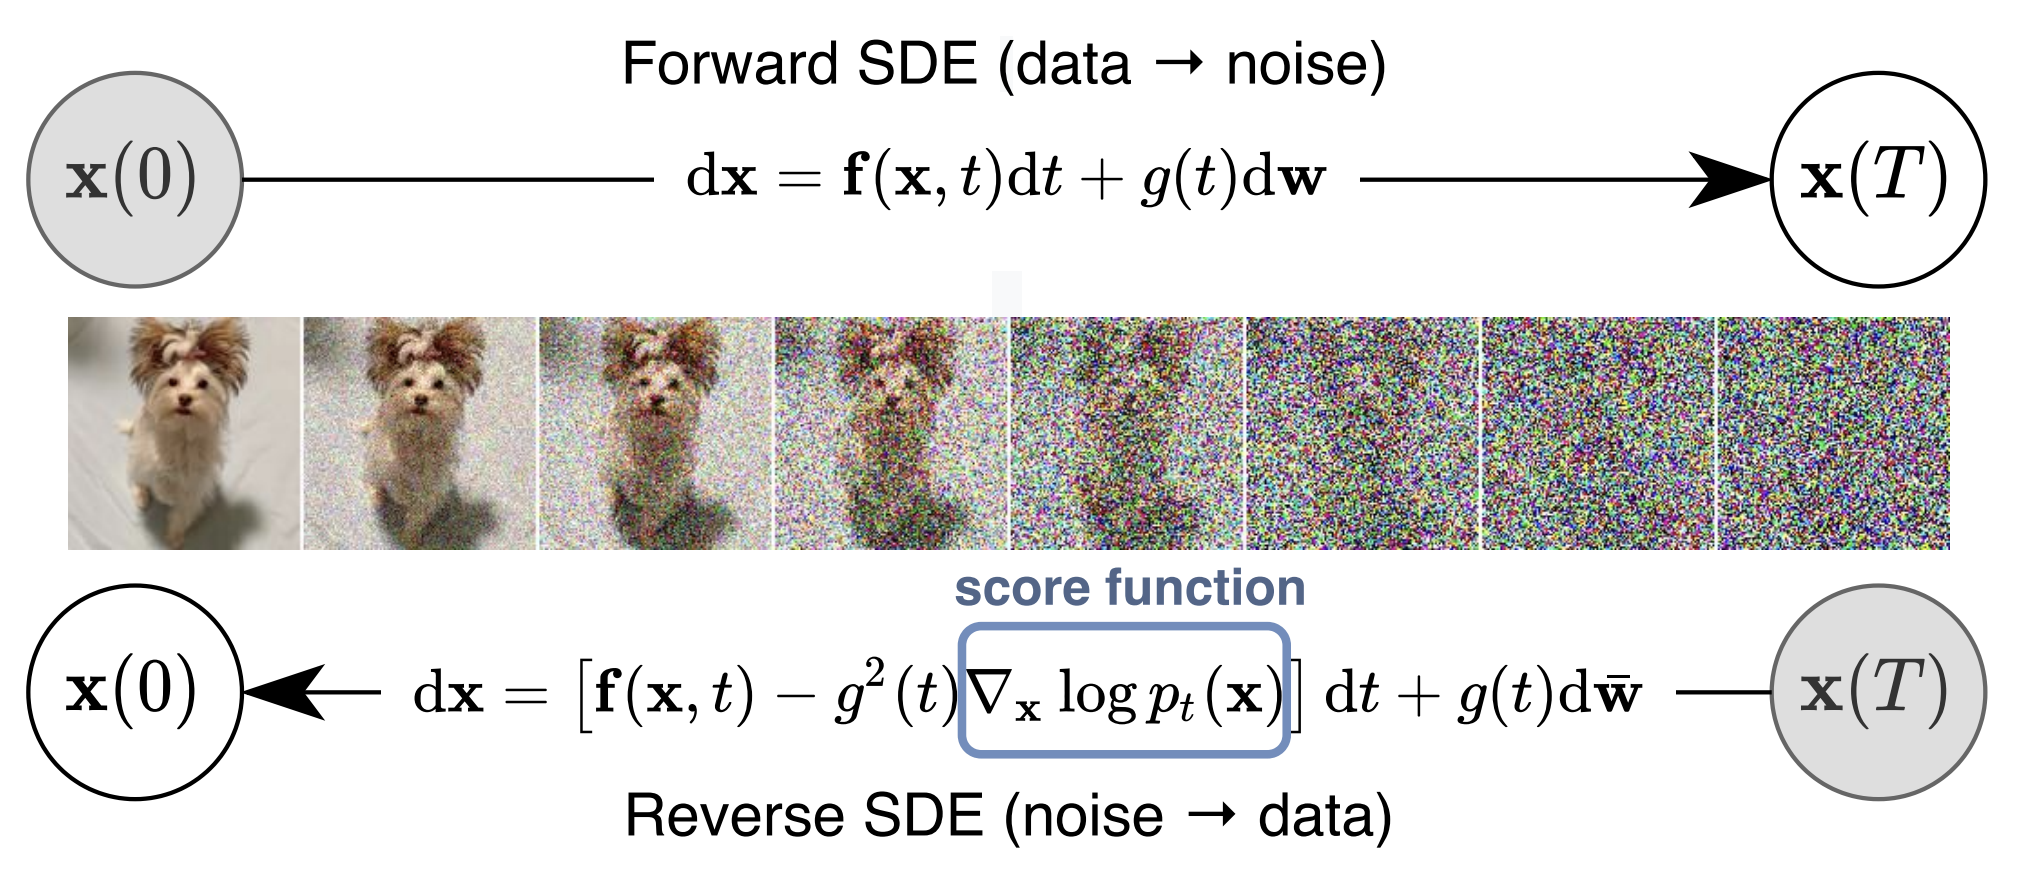
\includegraphics[width=0.8\linewidth]{figs/sbgm}
		\end{figure}
		\vspace{-0.5cm}
	\end{block}
    \eqpause
	\begin{itemize}
		\item Discretizing the reverse SDE provides ancestral sampling.
		\item Discretizing the probability flow ODE yields deterministic sampling.
	\end{itemize}
\end{frame}
%=======
\section{Flow Matching (FM)}
%=======
\begin{frame}{Continuous-Time Normalizing Flows}
    \myfootnotewithlink{https://arxiv.org/abs/1806.07366}{Chen R. T. Q. et al. Neural Ordinary Differential Equations, 2018}   

	Let's return to ODE dynamics $\bx_t = \bx(t)$ in the interval $t \in [0, 1]$:
	\begin{itemize}
		\item $\bx_0 \sim p_0(\bx)$, where $p_0(\bx)$ is a base distribution (mostly $\cN(0, \bI)$);
		\item $\bx_1 \sim p_1(\bx)$, where $p_1(\bx)$ is the true data distribution $\pd(\bx)$.
	\end{itemize}
	\[
		\frac{d \bx_t}{dt} = \bv (\bx_t, t),  \quad \text{with initial condition } \bx(0) = \bx_0.
	\]
	The velocity $\bv$ determines a flow $\bpsi_t$: $\bx_t = \bpsi_t(\bx_0)$.
    \eqpause
	\begin{block}{KFP Theorem (Continuity Equation)}
		\vspace{-0.5cm}
		\[
			\frac{\partial p_t(\bx)}{\partial t} = - \diver\left(\bv(\bx, t) p_t(\bx)\right) \Leftrightarrow \frac{d \log p_t(\bx(t))}{d t} = - \tr \left( \frac{\partial \bv(\bx(t), t)}{\partial \bx(t)} \right)
		\]
		\vspace{-0.5cm}
	\end{block}
    \eqpause
	\begin{itemize}
		\item It's hard to solve the continuity equation directly due to the trace term.
		\item There's a method (the adjoint method) that solves this equation directly, but it's unstable and unscalable.
	\end{itemize}
\end{frame}
%=======
\begin{frame}{Continuous-Time Normalizing Flows}
    \myfootnotewithlink{https://arxiv.org/abs/2210.02747}{Lipman Y., et al. Flow Matching for Generative Modeling, 2022}
	\begin{block}{KFP Theorem (Continuity Equation)}
		\vspace{-0.5cm}
		\[
			\frac{\partial p_t(\bx)}{\partial t} = - \diver\left(\bv(\bx, t) p_t(\bx)\right) \Leftrightarrow \frac{d \log p_t(\bx(t))}{d t} = - \tr \left( \frac{\partial \bv(\bx(t), t)}{\partial \bx(t)} \right)
		\]
		\vspace{-0.3cm}
	\end{block}
	\begin{itemize}
		\item Knowing the vector field $\bv (\bx, t)$, the KFP (or continuity) equation allows us to compute the density $p_t(\bx)$.
		\item Flow matching provides scalable approach to Neural ODEs.
	\end{itemize}
    \eqpause
	\begin{block}{Flow Matching}
		\vspace{-0.3cm}
		\[
			\bbE_{t \sim U[0, 1]} \bbE_{\bx \sim p_t(\bx)}\left\| \bv(\bx, t) - \bv_{\btheta}(\bx, t) \right\|^2 \rightarrow \min_{\btheta}
		\]
		\vspace{-0.3cm}
	\end{block}
    \eqpause
	\begin{itemize}
		\item Approximate the true vector field $\bv (\bx, t)$ using $\bv_{\btheta}(\bx, t)$.
		\item Use the learned flow $\bpsi_t$ for deterministic sampling: $\bx_1 = \bpsi_1(\bx_0)$.
	\end{itemize}
\end{frame}
%=======
\begin{frame}{Flow Matching: Training and Sampling}
	\myfootnotewithlink{https://arxiv.org/abs/2210.02747}{Lipman Y., et al. Flow Matching for Generative Modeling, 2022}
	\[
		\bbE_{t \sim U[0, 1]} \bbE_{\bx \sim p_t(\bx)}\left\| \bv(\bx, t) - \bv_{\btheta}(\bx, t) \right\|^2 \rightarrow \min_{\btheta}
	\]
	\[
		\bx_0 \sim p_0(\bx) = p(\bx), \quad \bx_1 \sim p_1(\bx) =  \pd(\bx)
	\]
	\eqpause
	\vspace{-0.3cm}
	\begin{block}{Training}
		\begin{enumerate}
			\item Sample $t \sim U[0, 1]$, $\bx_t \sim p_t(\bx)$.
			\item Compute loss $ \cL = \left\| \bv(\bx_t, t) - \bv_{\btheta}(\bx_t, t) \right\|^2 $.
		\end{enumerate}
	\end{block}
	\eqpause
	\begin{block}{Sampling}
		\begin{enumerate}
			\item Sample $\bx_0 \sim \cN(0, \bI)$.
			\item Solve the ODE to obtain $\bx_1$:
			\vspace{-0.3cm}
			\[
				\bx_1 = \bpsi_1(\bx_0) = \ODESolve_v(\bx_0, \btheta, t_0=0, t_1=1).
			\]
		\end{enumerate}
	\end{block}
	\vspace{-0.3cm}
	\eqpause
	\textbf{Problem:} The true vector field $\bv(\bx, t)$ is \textbf{unknown}.
\end{frame}
%=======
\begin{frame}{Flow Matching}
    \myfootnotewithlink{https://dl.heeere.com/conditional-flow-matching/blog/conditional-flow-matching}{image credit: A Visual Dive into Conditional Flow Matching}
	\[
		\bbE_{t \sim U[0, 1]} \bbE_{\bx \sim p_t(\bx)}\left\| \bv(\bx, t) - \bv_{\btheta}(\bx, t) \right\|^2 \rightarrow \min_{\btheta}
	\]
	\vspace{-0.5cm}
	\begin{itemize}
		\item There are infinitely many possible $\bv(\bx, t)$ between $p_0(\bx)$ and $p_1(\bx)$.
		\item We need to select the "best" $\bv(\bx, t)$ and make the objective tractable.
	\end{itemize}
	\begin{figure}
		\centering
		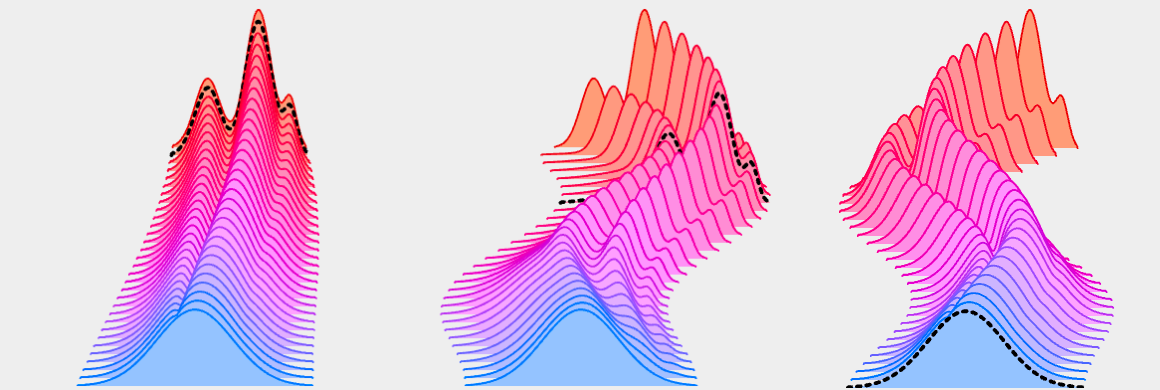
\includegraphics[width=\linewidth]{figs/multiple_dynamics}
	\end{figure}
\end{frame}
%=======
\begin{frame}{Summary}
	\begin{itemize}
		\item Score matching (NCSN) and diffusion models (DDPM) are discretizations of SDEs (variance exploding and variance preserving).
		\vfill
		\item Every SDE admits a corresponding probability flow ODE that follows the same probability path $p_t(\bx)$, yielding deterministic invertible sampling and exact log-likelihoods via the instantaneous change of variables.
		\vfill
		\item Converting SDEs to PF-ODEs enables efficient high-order numerical solvers, reducing the number of inference steps from $100$--$1000$ to $20$--$50$.
		\vfill
		\item SDEs can be reversed in time using the score function $\nabla_{\bx} \log p_t(\bx)$; discretizing the reverse SDE gives ancestral sampling, while discretizing the PF-ODE gives deterministic sampling.
		\vfill
		\item The continuous-time score matching objective generalizes DDPM and NCSN; for affine-drift SDEs the transition kernel $q(\bx(t) | \bx(0))$ is Gaussian, making the training objective tractable.
		\vfill
		\item Flow matching fits the vector field $\bv(\bx, t)$ directly, an alternative parametrization of the same continuous-time generative dynamics.
	\end{itemize}
\end{frame}
\end{document}